\PassOptionsToPackage{hyphens}{url}
\documentclass[12pt,onecolumn]{elsarticle}
\usepackage[T1]{fontenc}
\usepackage[utf8]{inputenc}

% Package structure from Computational Condensed Matter
\usepackage{lineno,hyperref}
\modulolinenumbers[7]
\usepackage{graphicx}
\usepackage{multirow}
\usepackage{dcolumn}% Align table columns on decimal point
\usepackage{epsfig}
\usepackage{amssymb}
\usepackage{amsmath}
\usepackage{bm}% bold math
\usepackage{bibtopic}
\usepackage{subfigure}
\usepackage{xcolor}
\usepackage[normalem]{ulem}

% Additional dependencies required for perovskite paper tables
\usepackage{booktabs}
\usepackage{tabularx} % Added for text-wrapping columns
\usepackage{array}    % For custom column formatting
\usepackage{longtable}% For multi-page tables
\usepackage[hyphens]{url}
\usepackage{float} % Added for exact float placement with [H]

\journal{Computational Condensed Matter}
\bibliographystyle{elsarticle-num}

\begin{document}

\begin{frontmatter}

\title{Interpretable Machine Learning and Symbolic Regression for Predicting Electronic, Magnetic, and Thermodynamic Properties of Double Perovskites}

\author{Nihal Gazi}
\author{Meghneel Ghosh}
\author{Subarna Datta\corref{cor1}}
\ead{subarna.iem87@gmail.com}
\author{Soumyadipta Pal\corref{cor1}}
\ead{soumyadipta.pal@gmail.com}

\cortext[cor1]{Corresponding authors}
\address{Institute of Engineering \& Management, Management House, D-1, Sector-V, Saltlake Electronics Complex, Kolkata-700091, India}
\address{University of Engineering and Management, New Town, University Area, Plot No. III, B/5, New Town Rd, Action Area III, Newtown, Kolkata-700160,India}


\begin{abstract}
Exploring the high-dimensional compositional space of double perovskites ($A_2BB'O_6$) using density functional theory (DFT) is computationally demanding. Materials informatics models can accelerate discovery, but black-box machine learning approaches lack physical interpretability. In this work, we present an interpretable hybrid machine learning pipeline to autonomously discover physical equations governing the properties of double perovskites. Using unsupervised Variational Autoencoders (VAEs) and $t$-SNE, we project eight target physical properties onto a three-dimensional latent manifold, revealing smooth physical gradients that establish learnable property mappings. We benchmark baseline linear regressions (OLS, Ridge, Lasso) against Gradient Boosting Trees to establish upper predictability limits. To resolve these black-box models, we employ Symbolic Regression (Genetic Programming) guided by tree-based feature importances to search for clean, factorable algebraic equations. The pipeline successfully discovers a novel electronic-geometric custom tolerance factor for formation energy ($\Delta E_f$) and captures the structural-magnetic coupling of total magnetization ($M$), matching the performance of black-box tree models. Our analysis of electronic band gaps ($E_g$) highlights the intrinsic limitations of machine learning on under-relaxed DFT data. This framework demonstrates a robust methodology for white-box physical law discovery directly from crystal structure geometries.
\end{abstract}

\begin{keyword}
Double perovskites \sep Symbolic regression \sep Machine learning \sep Density functional theory \sep Materials informatics \sep Variational autoencoders
\end{keyword}

\end{frontmatter}

\section{Introduction}
Perovskite compounds have been of extreme interest in the recent years in the field of material sciences. Owing their extreme versatility and unusually wide range of applications – they have gained significant attention in the scientific community. This specifically structured compound has demonstrated behaviors such as that solar cell, LEDs, memory device, sensors and even quantum materials \cite{green2014emergence, pacchioni2021highly, gu2016flexible, li2025design, nguyen2021hexagonal, ali2024elastic}.

Perovskites have the same lattice structure, however, changing their atoms heavily influences their physical and chemical properties. They have the formula ABX3. Double perovskites are structural derivatives of the standard $ABX_3$ lattice, characterized by an alternating rock-salt arrangement of two distinct transition metals, yielding the formula $A_2BB'X_6$. The additional central atom allows it for an even wider variety of materials.

However, a central problem, before working with a perovskite material, is analysis of their various properties, such as, Energy above hull, bandgap, total magnetization and formation energy, as experimentally finding these values costs time and requires precise experiments and hardware, which often becomes a hurdle, before any material science analysis could be made. Historically, the design and discovery of novel double perovskite oxides ($A_2BB'O_6$) have relied on empirical heuristics, such as the Goldschmidt Tolerance Factor ($t$) and the octahedral mismatch ratio ($\mu_{\text{oct}}$) \cite{goldschmidt, shannon}. These 1D structural descriptors relate ionic sizes to structural stability, but they are insufficient for predicting complex electronic or magnetic ground states.

The present state-of-the-art method for evaluating various optical, mechanical, thermodynamic and structural properties uses the Density Functional Theory(DFT) \cite{nguyen2021hexagonal, jamshaid2023investigation}. DFT uses a series of highly complex and expensive algorithms to predict electron cloud density distribution over any 3D lattice of a chemical compound. This framework has been used, in the past decade, to generate high-throughput DFT databases, such as the Materials Project \cite{materialsproject}, which has enabled data-driven materials discovery by providing thousands of relaxed crystal structures and corresponding thermodynamic properties.

The traditional DFT framework, while highly accurate, is extremely costly in terms of time and processing power. Recently, however, through combination of machine learning and deep learning, material scientists have been able to predict structural, optical, mechanical and thermodynamic properties to a considerably high accuracy.

Hence, deep learning architectures, particularly Crystal Graph Neural Networks (CGNNs), have revolutionized the field by directly encoding 3D atomic coordinates and cell topologies of perovskites\cite{zhang2025efficient}. They learn localized atomic interactions, enabling the prediction of energy landscapes and forces. However, despite being more efficient than DFT, CGNNs require large training sets and operate as black boxes, making it difficult to extract the underlying physical principles governing their predictions. 

In this paper, we use a combination of certain algorithms and find interpretable exact mathematical formulae using Machine Learning techniques that is both readable by humans and aligns to chemical data. We explore various other features to find mathematical models, that are highly interpretable and ultimately conclude the feasibility and scalability of our pipeline. We report the results we found, and how accurately they align with real world data.

We deploy a structured 4 stage analysis pipeline. At Stage 1, we extract all relevant Quantum Data pertaining to the perovskite that deemed to be necessary irrespective of how relevant they may be. At Stage 2, we do a hyperdimensional analysis of visual trends through Deep unsupervised learning inorder to identify deeper trends that may be missed due to human error. At Stage 3, We discover the weightage of each properties through machine learning algorithms. At Stage 4, we use all the collected data, and run it through Symbolic Regression and Linear Regression to search for an accurate mathematical equation, that describes the given dataset, in reasonable time through search space reduction.

\section{Methodology}

\subsection{Data Collection}

The data was extracted through the Materials Project database \cite{materialsproject}. The Formation Energy (eV/atom), Energy Above Hull (eV), Band Gap (eV), and Total Magnetization ($\mu_B$) values were extracted from the Material Project’s computational records that were calculated using Density Functional Theory (DFT) \cite{materialsproject}. These were passed through a rigorous filtering process involving crystallographic, geometric, and compositional heuristics – which were again cross-verified against established chemical literature \cite{goldschmidt, shannon} to confidently classify the compounds into double perovskites. The rest compounds which did not match the criteria were therefore labelled as non-true double perovskites.

This rigorous data collection procedure generated a 416 element dataset of double perovskite compounds. For each of these compounds, the baseline dataset included the chemical formula, space group symmetries, and the B/B'-site transition metals alongside their respective metallic radii. This dataset was then passed for further analysis as it avoided noisy data for the ML models, which are usually less robust to noise.

Furthermore, external data sources were used, such as the Mendeleev Database (for atomic electronegativities and shannon ionic radii) \cite{goldschmidt, shannon}, Materials Project REST API (for 3D crystal structure ) \cite{materialsproject}, PyMatgen (for calculating unit cell volumes, densities, Goldschmidt Tolerance Factors and Octahedral Mismatches) and a pre-trained CHGNet network to obtain relaxed atomic energies and magnetic spin configurations \cite{chgnet}.

The complete curated dataset utilized for this study is provided as Supplementary Material. Furthermore, to ensure full reproducibility, all machine learning pipelines, feature extraction scripts, and parsed data are openly available in our GitHub repository (\url{https://github.com/nihal-gazi/double-perovskite-interpretable-ml}).




\subsection{Stage 1: Gathering Physical and Quantum Descriptors}
Before running prediction, we needed additional data, that was not available from the available dataset. A good feature selection improves the model, hence, we proceeded with collecting as many features as possible irrespective of their potential contribution to final property prediction.

1. Mendeleev Database: The Mendeleev database can be imported through Python as a library, allowing for easy data retrieval for various atom and their properties. We sourced specifically Electronegativities and Shannon ionic radii for our experiment \cite{goldschmidt, shannon}.

2. Materials Project REST API: We extracted 3D crystal structure files for all double perovskites present in the dataset for further feature extraction. And unit cell volumes, densities, Goldschmidt Tolerance Factors ($t$), and Octahedral Mismatches ($\mu_{\text{oct}}$) were calculated using the PyMatgen library \cite{materialsproject}.

3. CHGNet: A pre-trained network called the CHGNet was used to obtain relaxed atomic energies ($E_{\text{GNN}}$) and magnetic spin configurations ($M_{\text{net}}$, $M_{\text{abs}}$) \cite{chgnet}. This network took input the 3D crystal structrues that we obtained from Materials Project REST API, and generates magnetic moments.

To ensure clarity regarding all the descriptors and physical quantities analyzed across these stages, Table \ref{tab:legend} provides a complete legend of all variables, symbols, and sources.

\begin{longtable}{l p{0.37\textwidth} p{0.34\textwidth}}
\caption{Comprehensive Physical Variables, Symbols, and Sources Legend}
\label{tab:legend} \\
\toprule
\textbf{Symbol} & \textbf{Physical Description \& Meaning} & \textbf{Sourcing / Extraction Method} \\
\midrule
\endfirsthead
\multicolumn{3}{c}%
{{\bfseries Table \thetable\ -- Continued from previous page}} \\
\toprule
\textbf{Symbol} & \textbf{Physical Description \& Meaning} & \textbf{Sourcing / Extraction Method} \\
\midrule
\endhead
\bottomrule
\endfoot
\bottomrule
\endlastfoot
\multicolumn{3}{l}{\textbf{Target Variables (DFT Ground-State Properties)}} \\
\midrule
$\Delta E_f$ or $E_f$ & Formation energy per atom (eV/atom); measures thermodynamic stability relative to pure elements. & Materials Project database \cite{materialsproject} \\
\addlinespace
$M$ & Total unit cell magnetization ($\mu_B$/f.u.); macroscopic net magnetic moment. & Materials Project database \cite{materialsproject} \\
\addlinespace
$E_{\text{hull}}$ & Energy above hull (eV/atom); thermodynamic stability relative to competing phases. & Materials Project database \cite{materialsproject} \\
\addlinespace
$E_g$ & Band gap (eV); electronic energy separation between valence and conduction bands. & Materials Project database \cite{materialsproject} \\
\midrule
\multicolumn{3}{l}{\textbf{Classical \& Geometric 1D Descriptors}} \\
\midrule
$t$ & Goldschmidt Tolerance Factor; geometric index of perovskite lattice stability: $t = \frac{r_A + r_O}{\sqrt{2}(r_{\text{avg}} + r_O)}$. & Calculated from Shannon ionic radii and cell topology via PyMatgen. \\
\addlinespace
$EN_{\text{avg}}$ & Average Pauling electronegativity of the B and B' site transition metals: $EN_{\text{avg}} = (EN_B + EN_{B'})/2$. & Looked up from Mendeleev database (atomic electronegativity tables). \\
\addlinespace
$\mu_{\text{oct}}$ & Octahedral mismatch ratio; measures size disparity between B and B' sites: $\mu_{\text{oct}} = r_B / r_{B'}$. & Looked up from Mendeleev database (Shannon ionic radii). \\
\addlinespace
$EN_X$ & Pauling electronegativity of the element occupying site $X \in \{A, B, B', O\}$. & Looked up from Mendeleev database. \\
\addlinespace
$Shannon_X$ / $r_X$ & Shannon ionic radius of the cation on site $X \in \{A, B, B'\}$ (\AA). & Sourced from Shannon ionic radii tables in Mendeleev database. \\
\addlinespace
$Val_{\text{avg}}$ & Average valence electron count of the transition metals occupying B and B' sites. & Sourced from Mendeleev database. \\
\midrule
\multicolumn{3}{l}{\textbf{3D Spatial \& GNN-Derived Quantum Features}} \\
\midrule
$d_{\text{avg}}$ & Average B--O and B'--O bond length in the relaxed crystal cell (\AA). & Parsed from crystal coordinates (.cif files) via PyMatgen. \\
\addlinespace
$d_{XO}$ & Individual octahedral bond length between site $X \in \{B, B'\}$ and oxygen (\AA). & Parsed from crystal coordinates (.cif files) via PyMatgen. \\
\addlinespace
$E_{\text{GNN}}$ & Relaxed total potential energy per atom (eV/atom). & Predicted via pretrained CHGNet GNN potential \cite{chgnet}. \\
\addlinespace
$M_{\text{abs}}$ & Sum of absolute local atomic magnetic moments ($\mu_B$). & Predicted via pretrained CHGNet GNN potential \cite{chgnet}. \\
\addlinespace
$M_{\text{net}}$ & Net unit cell magnetic moment ($\mu_B$). & Predicted via pretrained CHGNet GNN potential \cite{chgnet}. \\
\end{longtable}

\subsection{Stage 2: Visualizing Trends}
Before building predictive models, it is crucial to make sure that the data we are working has hidden patterns that can epxloited. We deployed a Variational Autoencoder, which is an unsupervised deep learning algorithm that learns to encode data into a smaller and compressed hyperdimensional latent vector containing high weightage abstract features which can later be reconstructed through the learned decoder.

For each perovskite compound, 8 features were considered: metallic radius 1, metallic radius 2, metallic radius 3, metallic radius 4, formation energy, energy above hull , band gap, and total magentization. The network was then compressed into a 3-Dimensional latent, ensuring a strong compression. The dataset points were then run through the Encoder and 3-Dimensional deep latent embeddings were generated for each perovskite. The embeddings were then visualized using t-SNE algorithm on a 2D Graph.

The analysis displayed trends that were clearly visible and understandable through human observation. Few trends displayed were highly noisy and were discarded. The generated graphs displayed are as follows:

\begin{figure}[H]
  \centering
  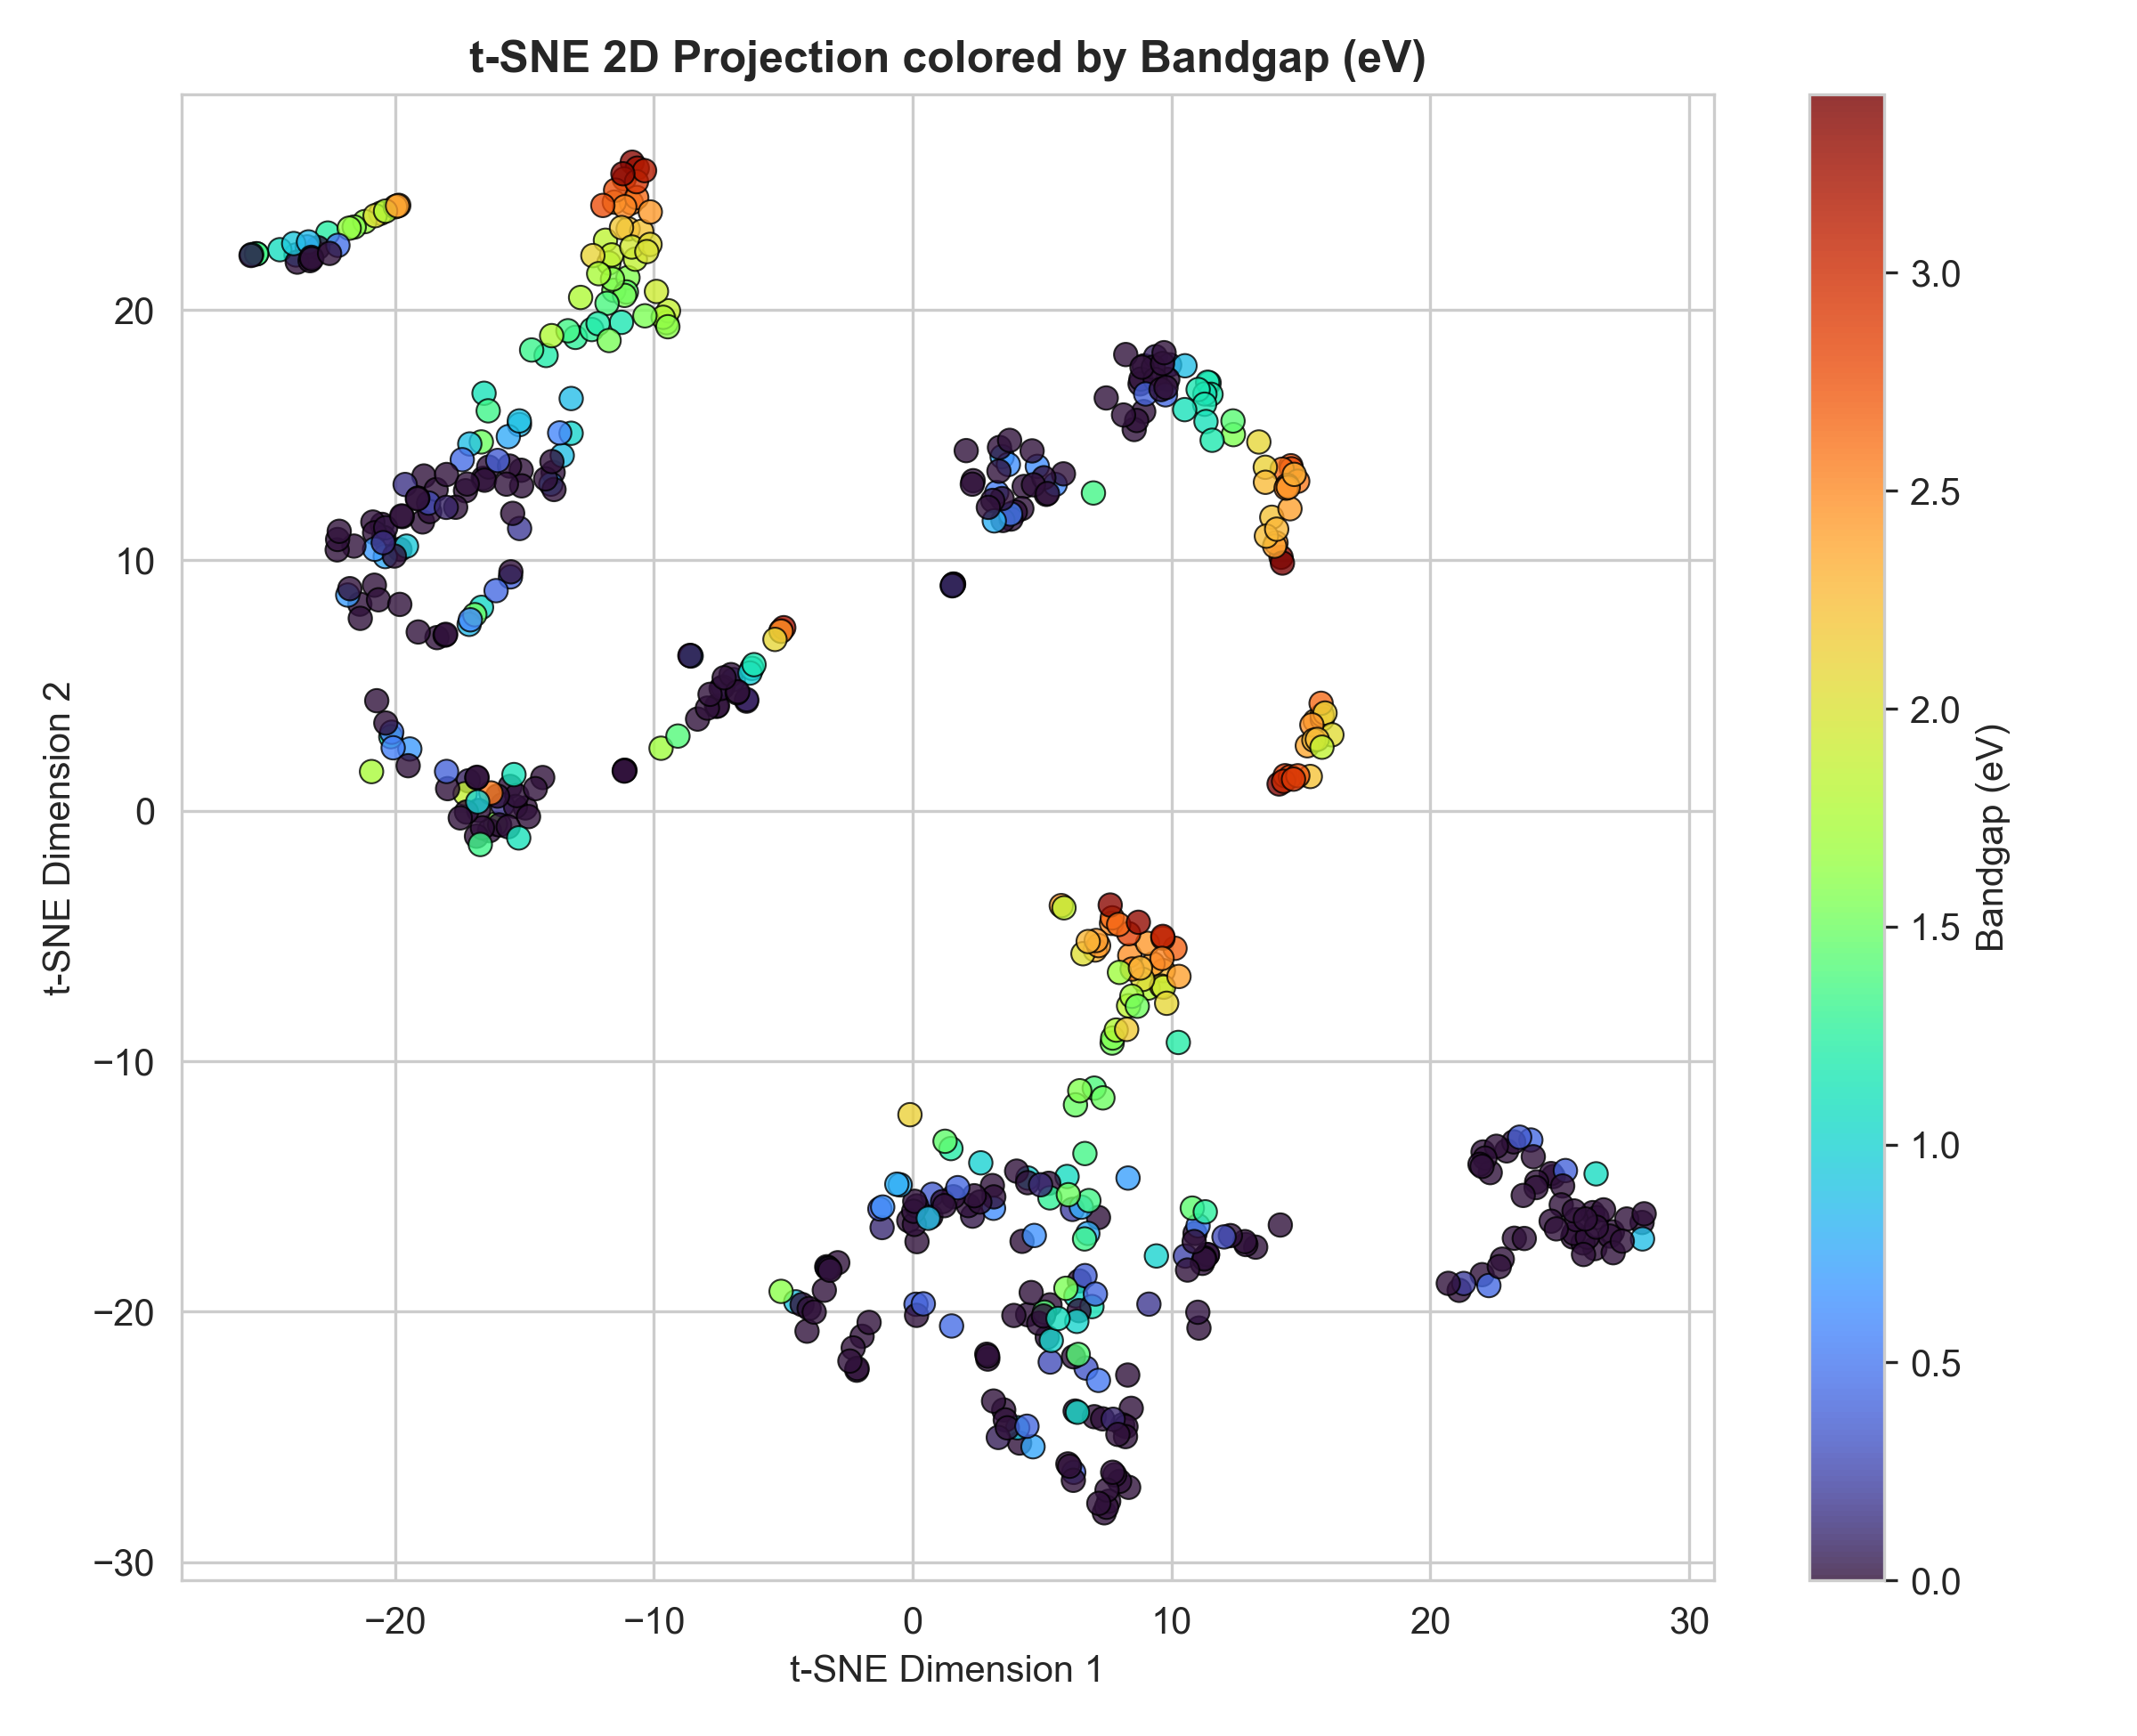
\includegraphics[width=0.65\textwidth]{3_2d_bandgap.png}
  \caption{t-SNE projection of the 3D VAE latent space colored by Bandgap (eV).}
  \label{fig:tsne_bandgap}
\end{figure}

\begin{figure}[H]
  \centering
  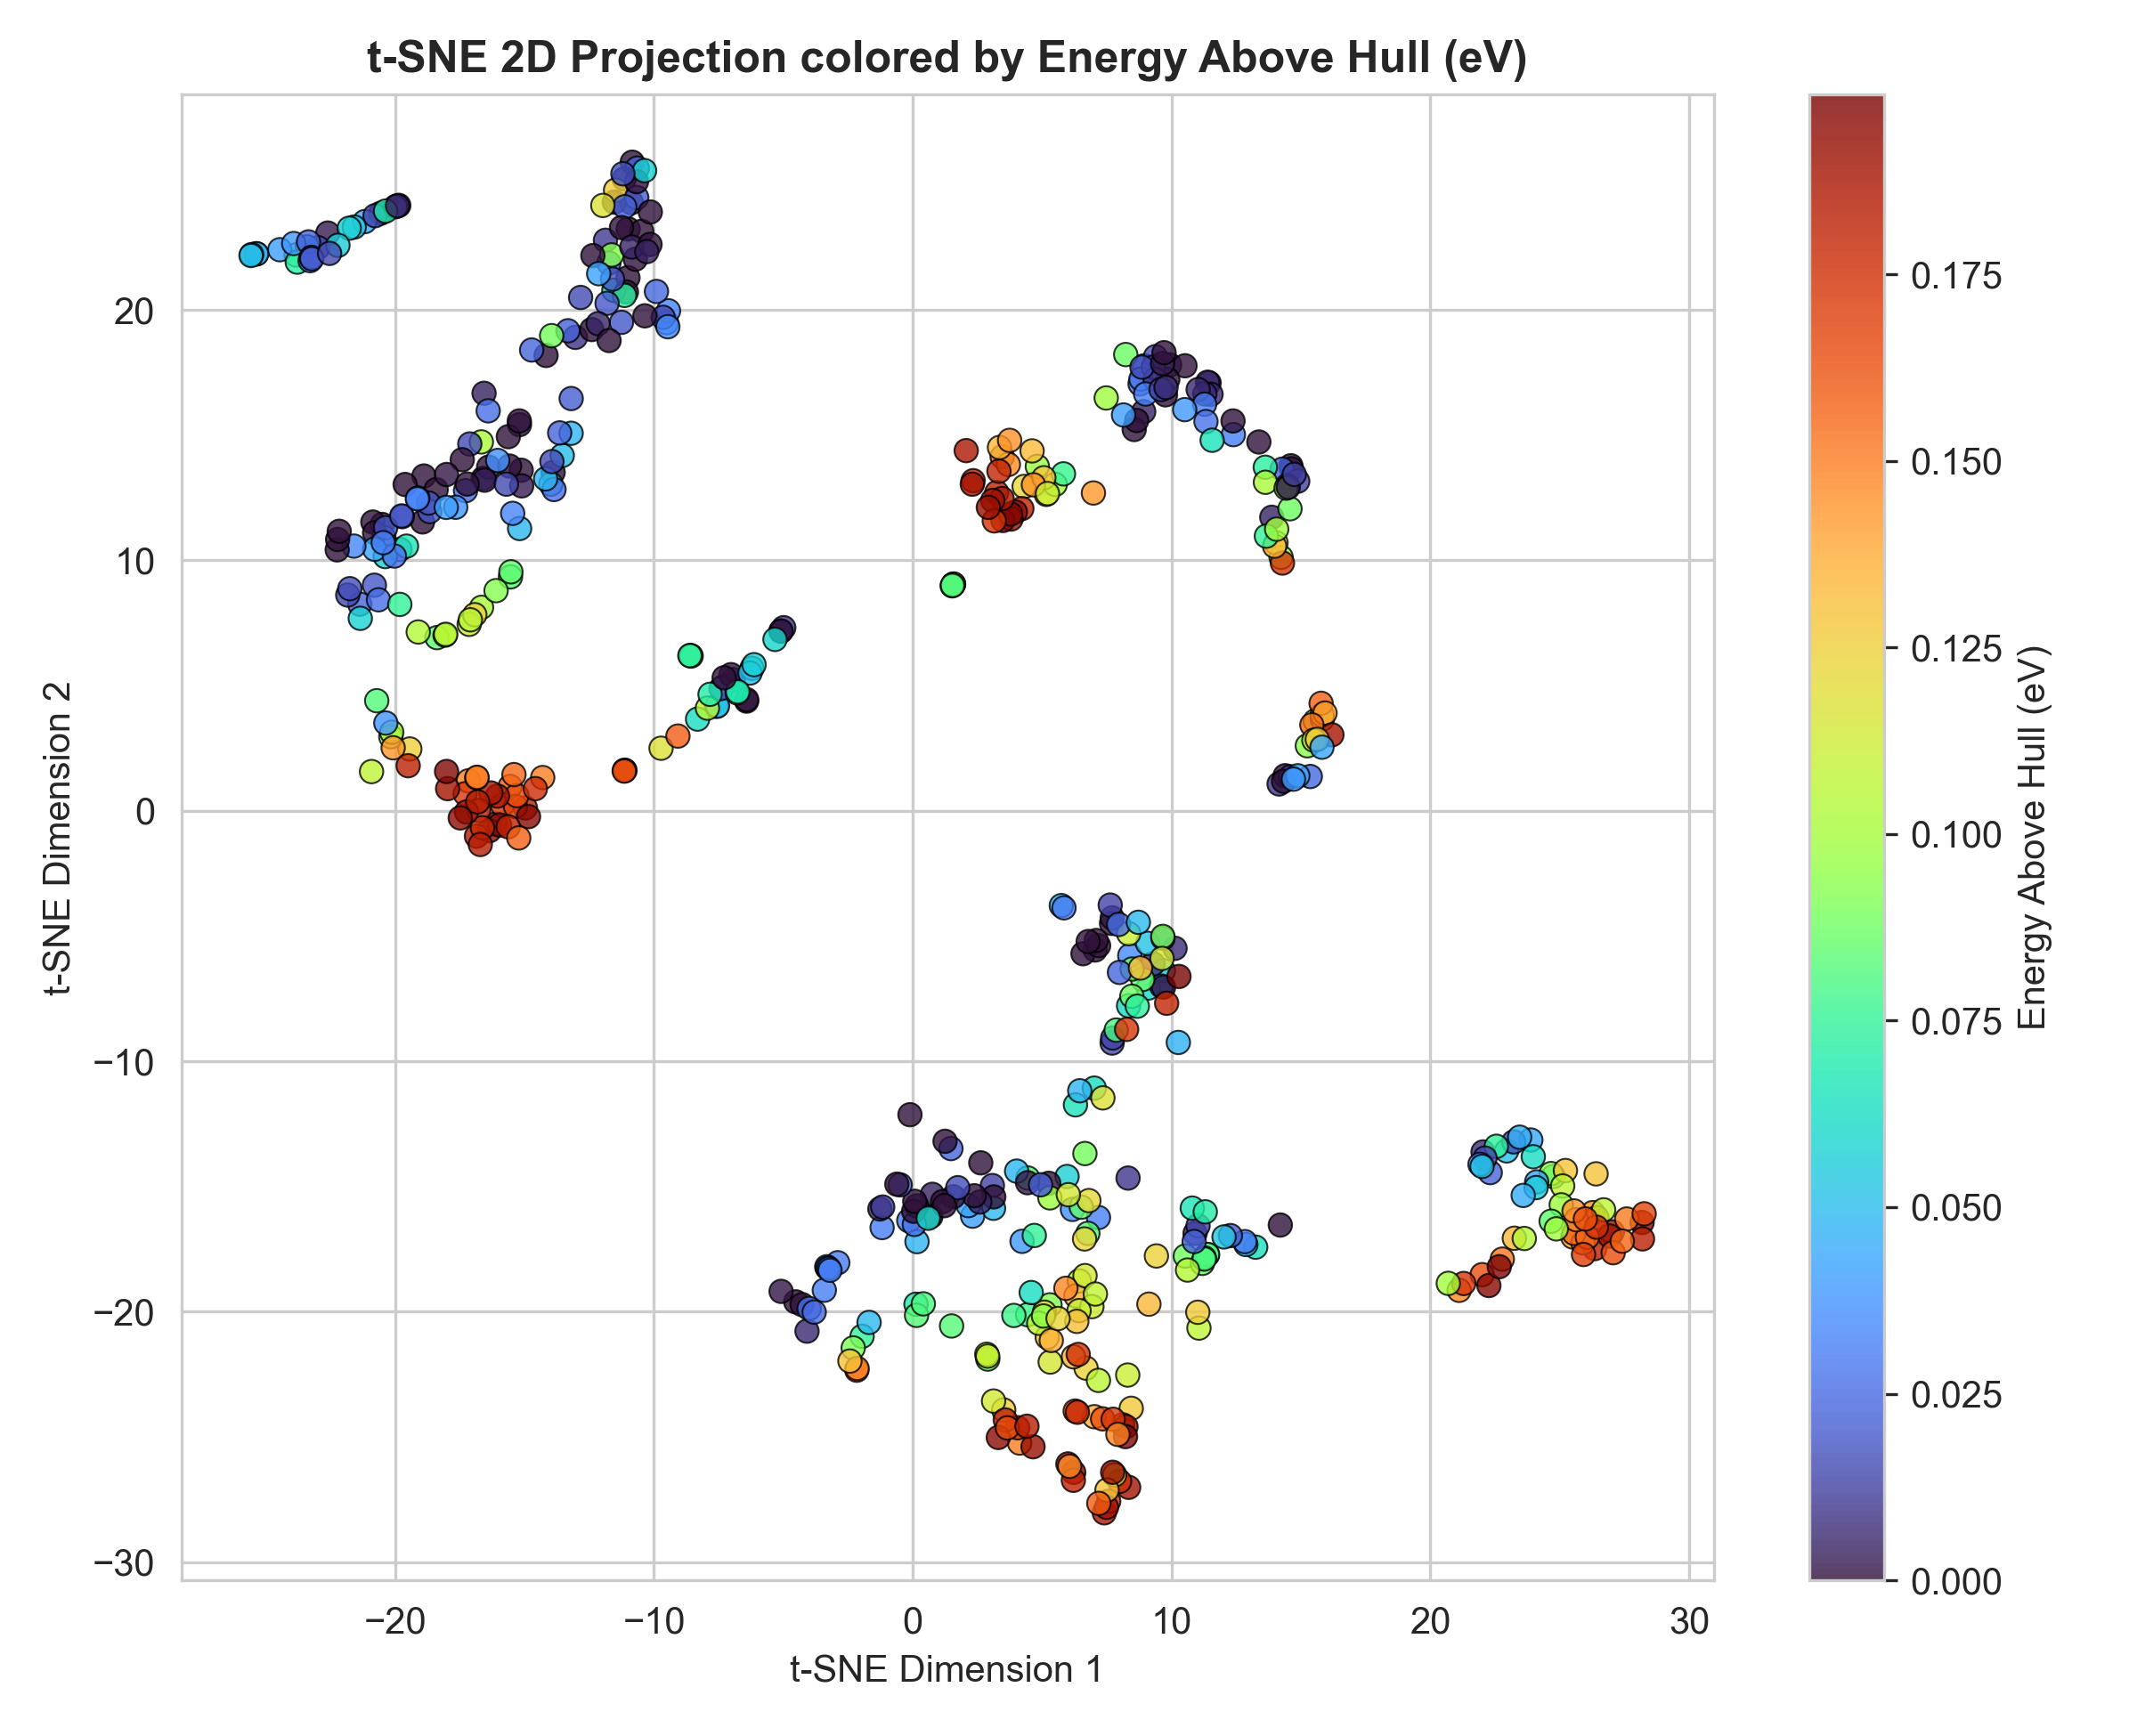
\includegraphics[width=0.65\textwidth]{3_2d_energy_above_hull.png}
  \caption{t-SNE projection of the 3D VAE latent space colored by Energy Above Hull (eV).}
  \label{fig:tsne_ehull}
\end{figure}

\begin{figure}[H]
  \centering
  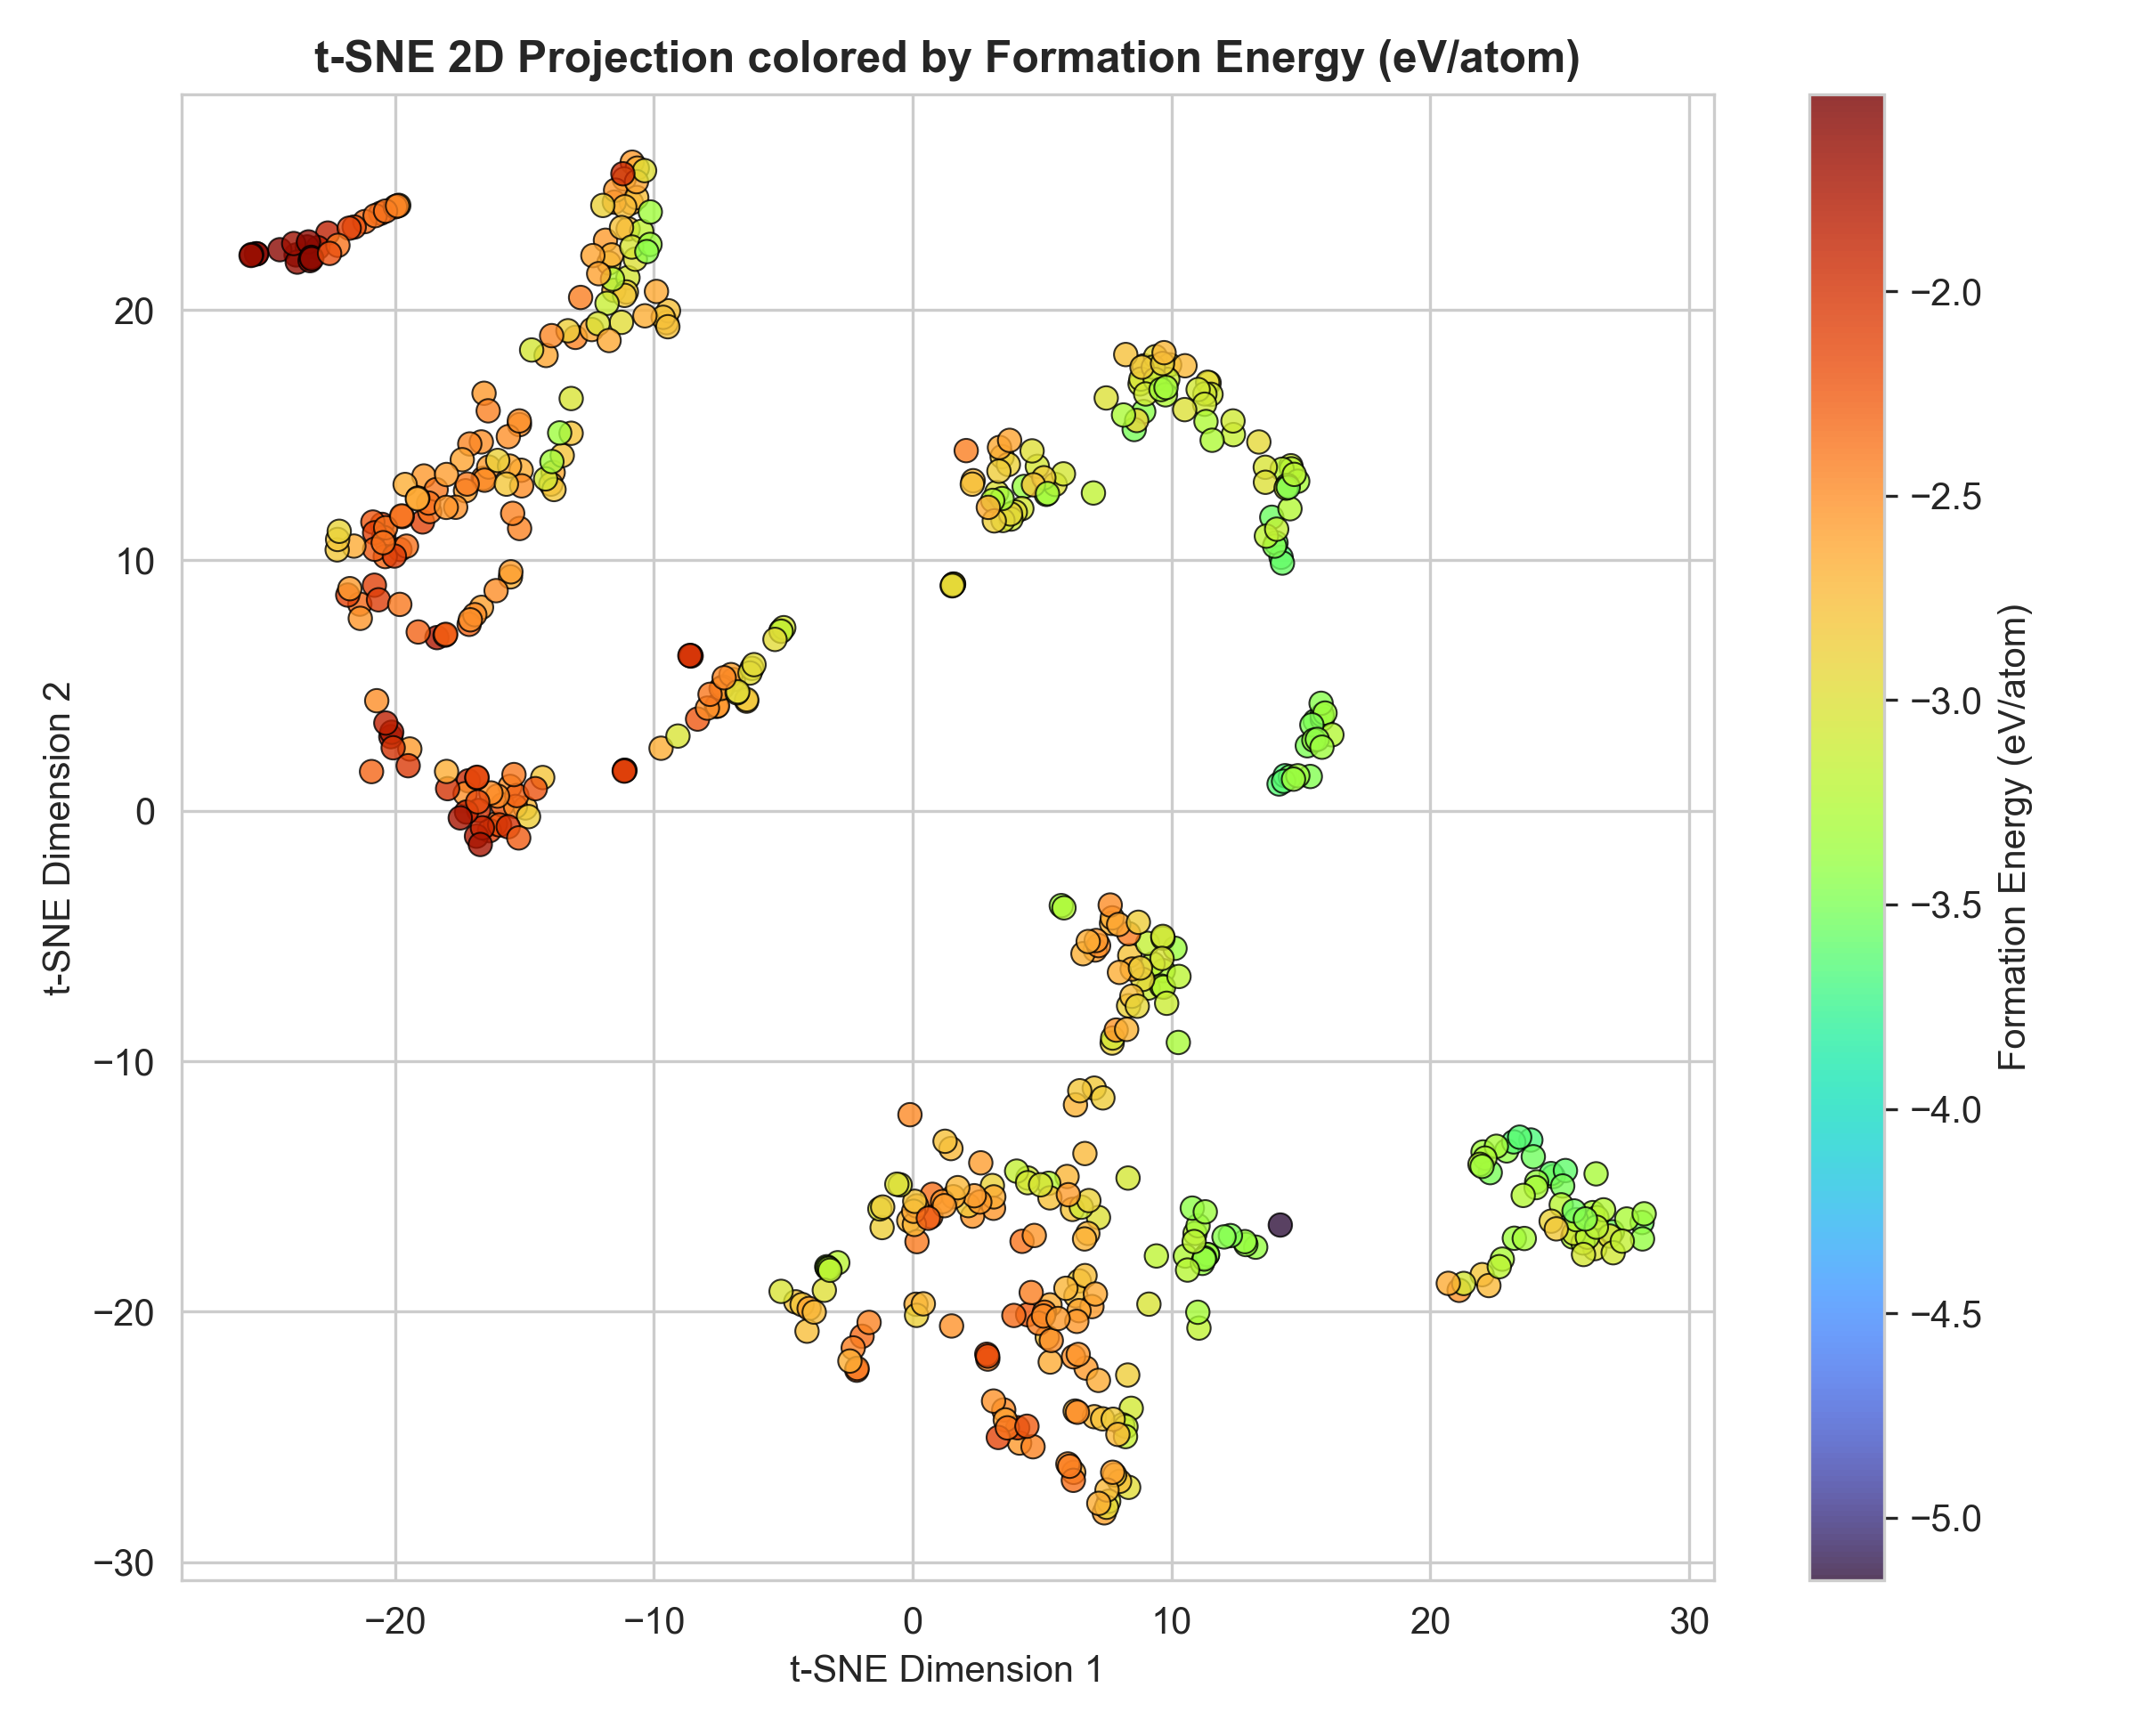
\includegraphics[width=0.65\textwidth]{3_2d_formation_energy.png}
  \caption{t-SNE projection of the 3D VAE latent space colored by Formation Energy (eV/atom).}
  \label{fig:tsne_ef}
\end{figure}

\begin{figure}[H]
  \centering
  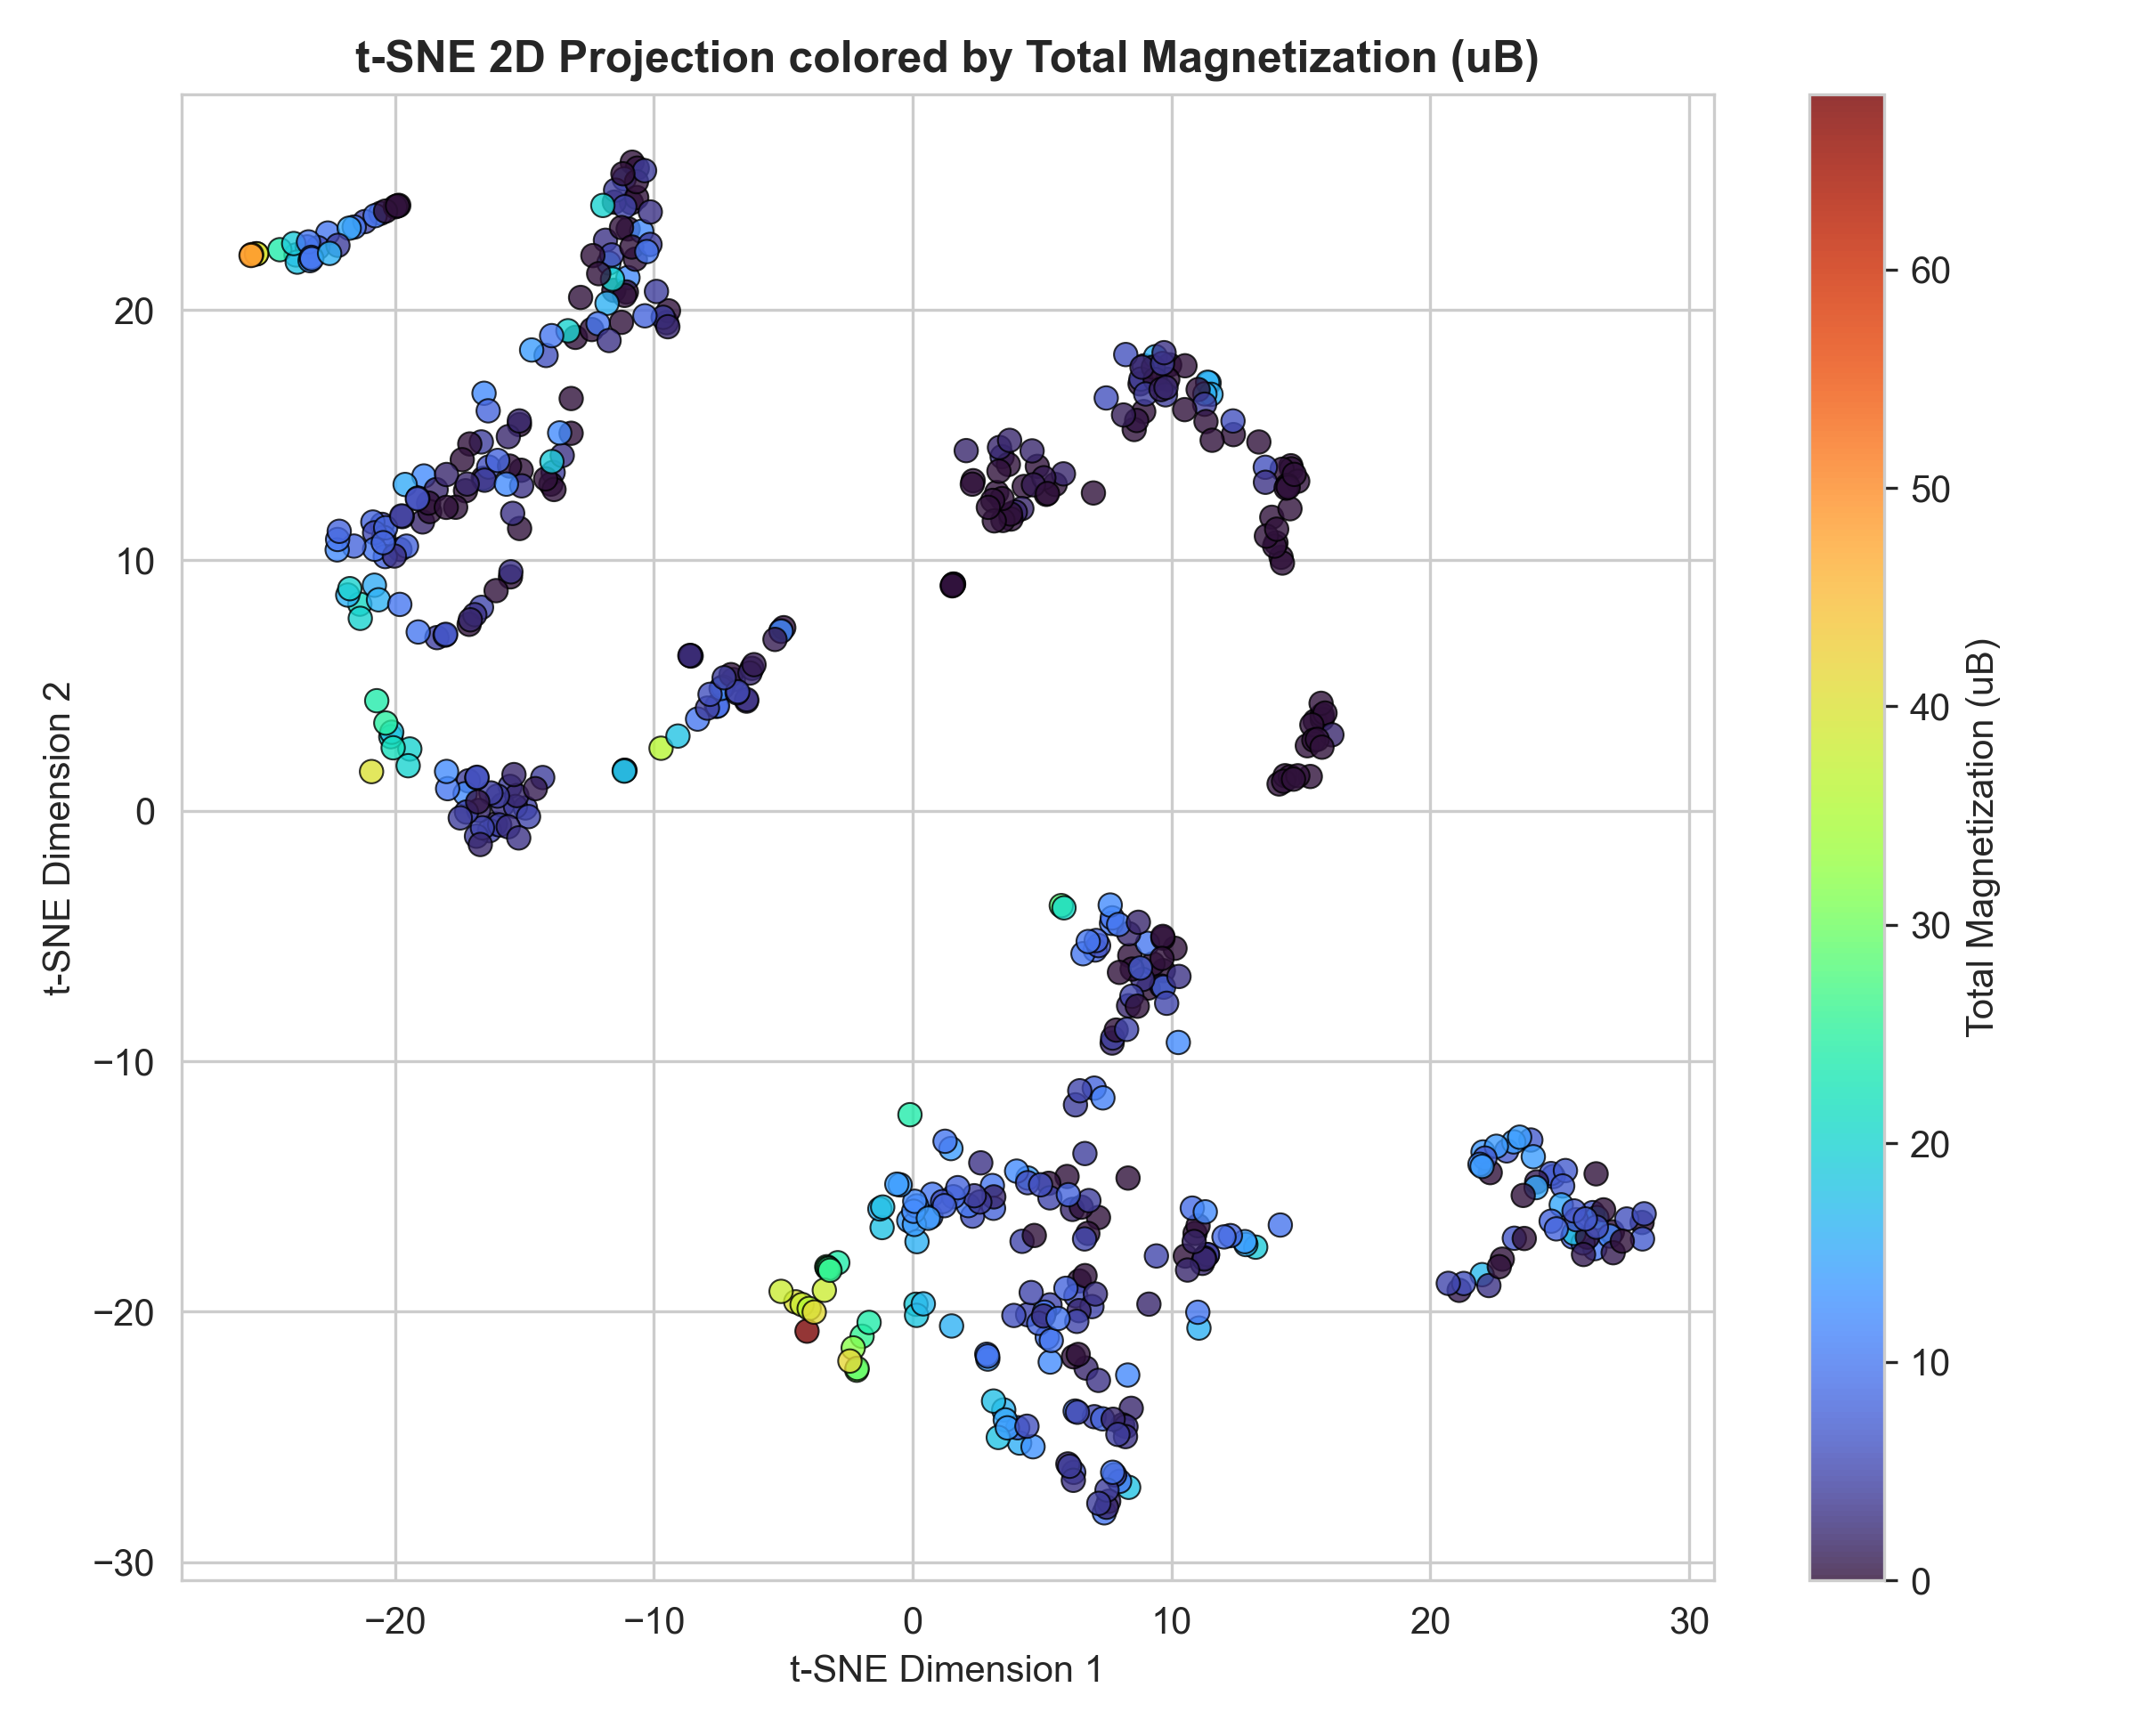
\includegraphics[width=0.65\textwidth]{3_2d_total_mag.png}
  \caption{t-SNE projection of the 3D VAE latent space colored by Total Magnetization ($\mu_B$).}
  \label{fig:tsne_mag}
\end{figure}

\begin{figure}[H]
  \centering
  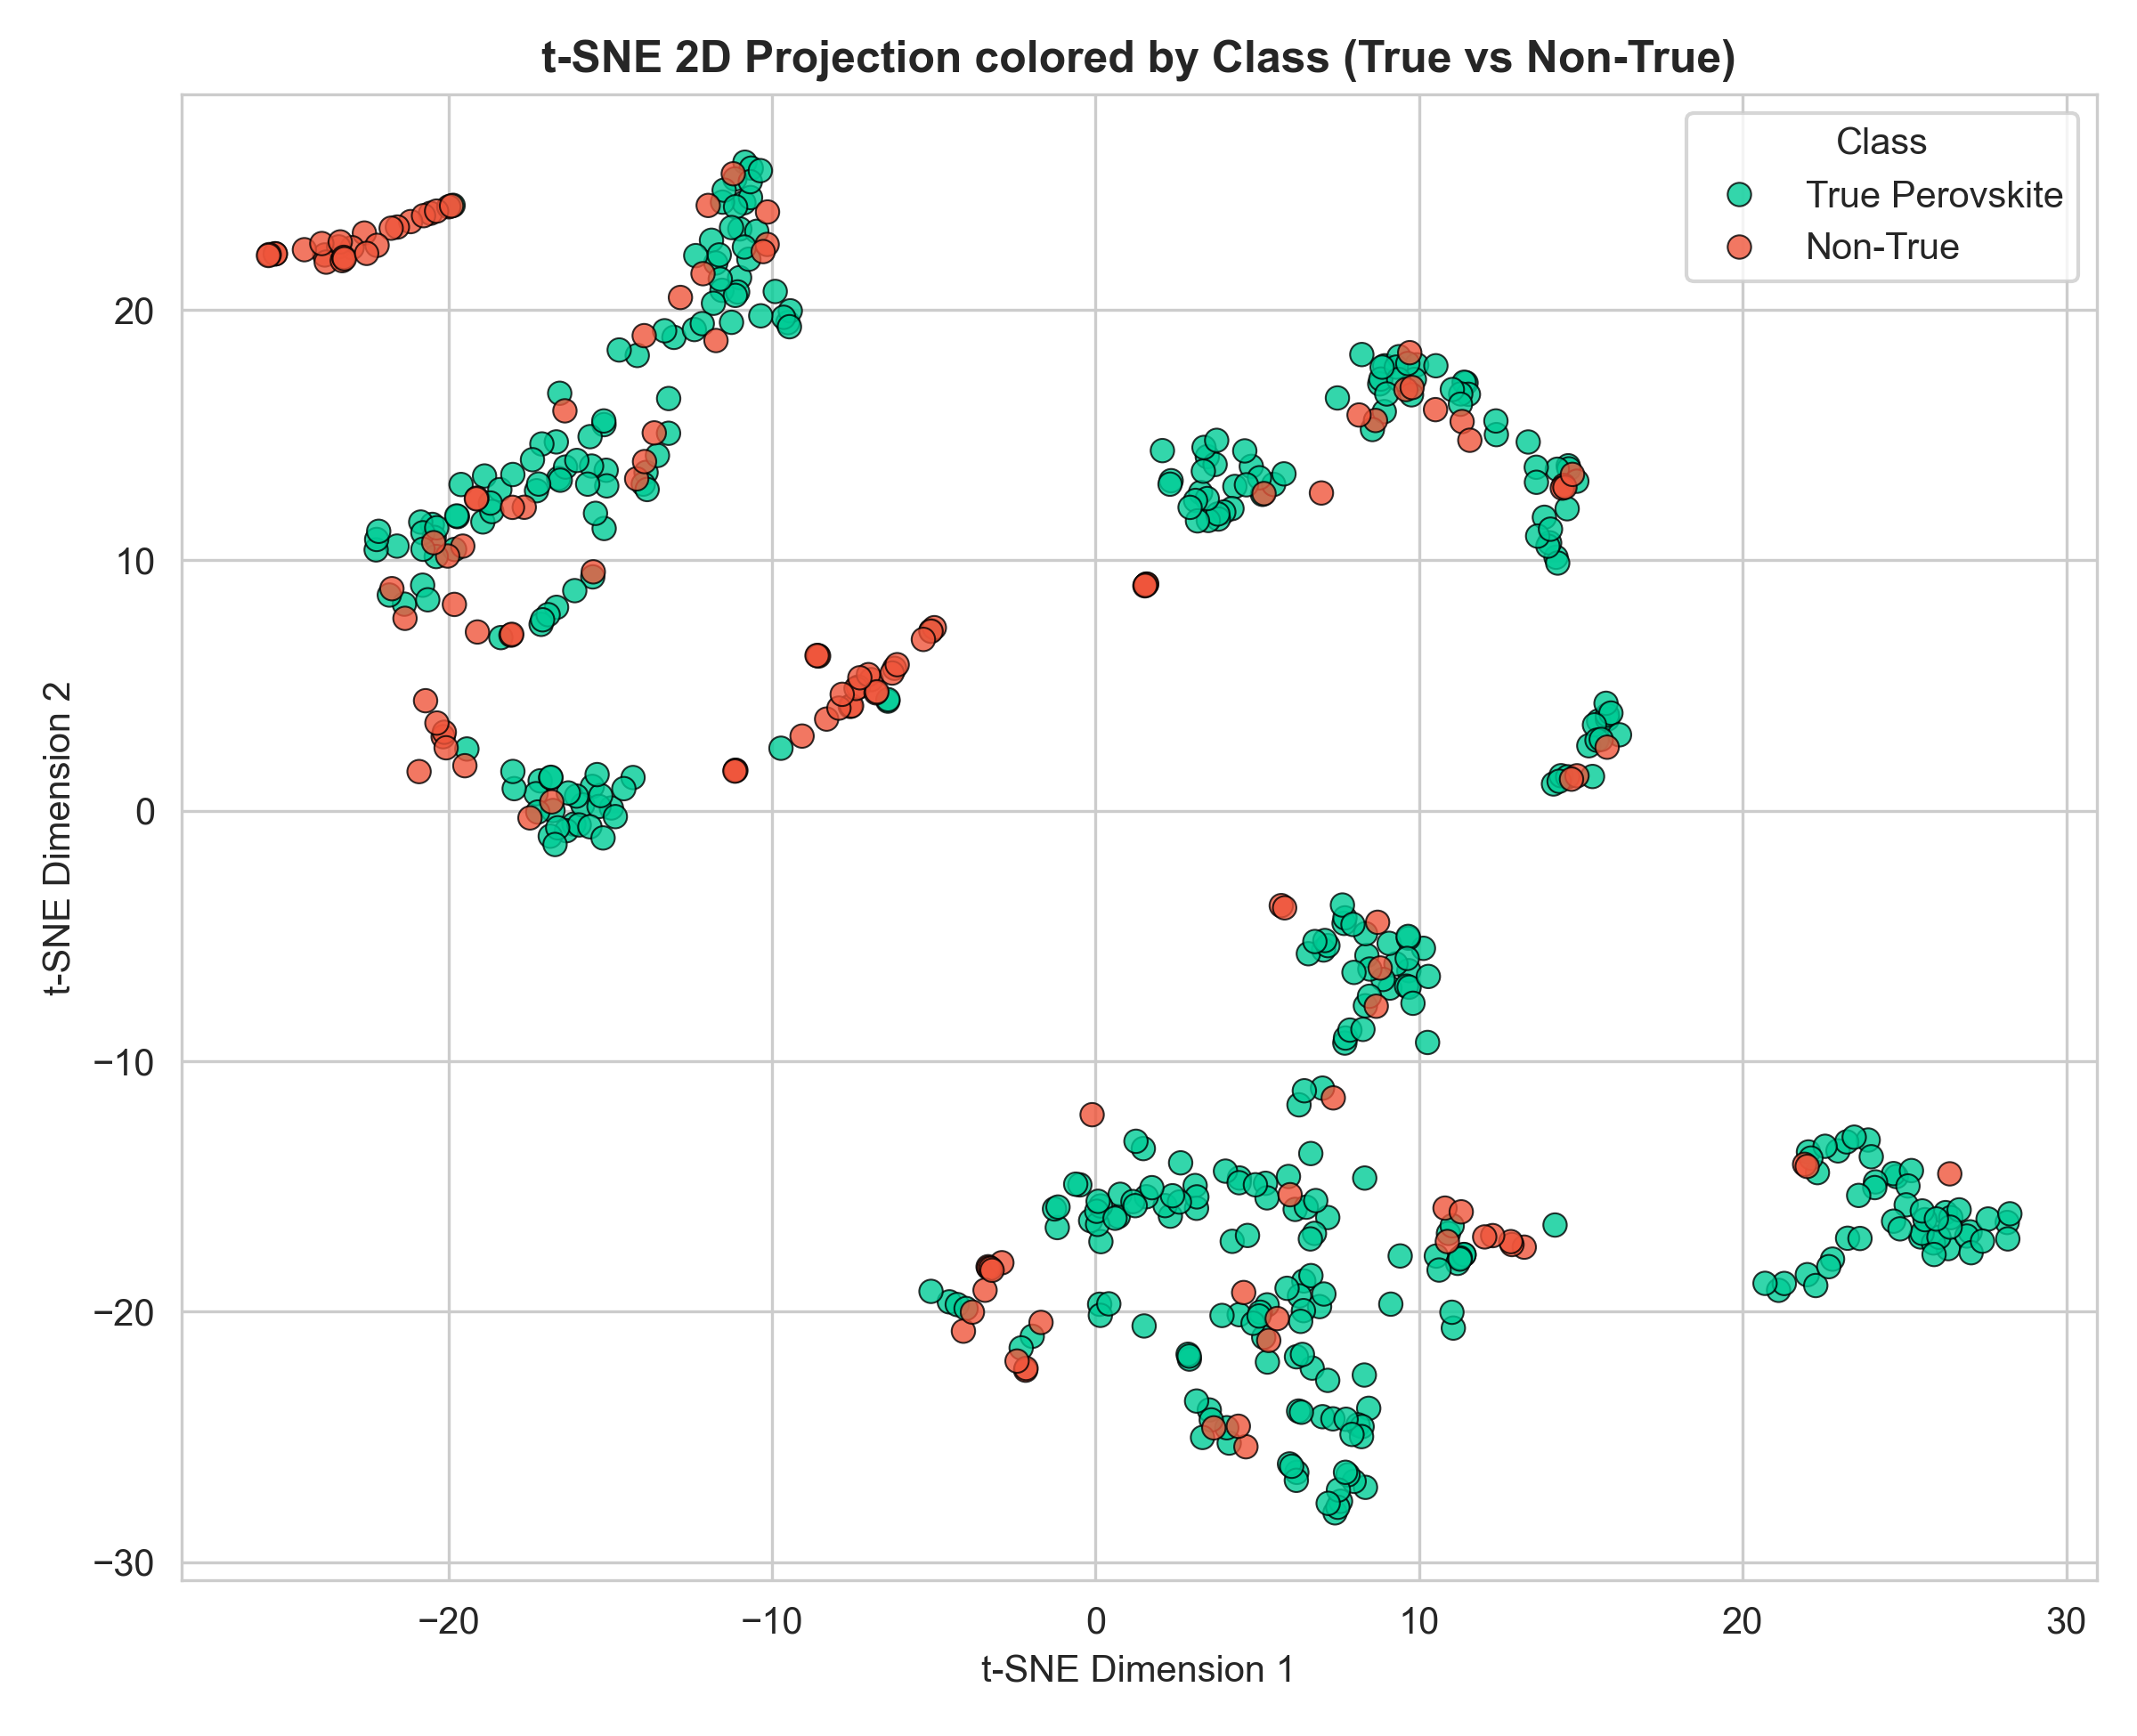
\includegraphics[width=0.65\textwidth]{3_2d_class.png}
  \caption{t-SNE projection of the 3D VAE latent space colored by Class (True vs Non-True).}
  \label{fig:tsne_class}
\end{figure}

\begin{figure}[H]
  \centering
  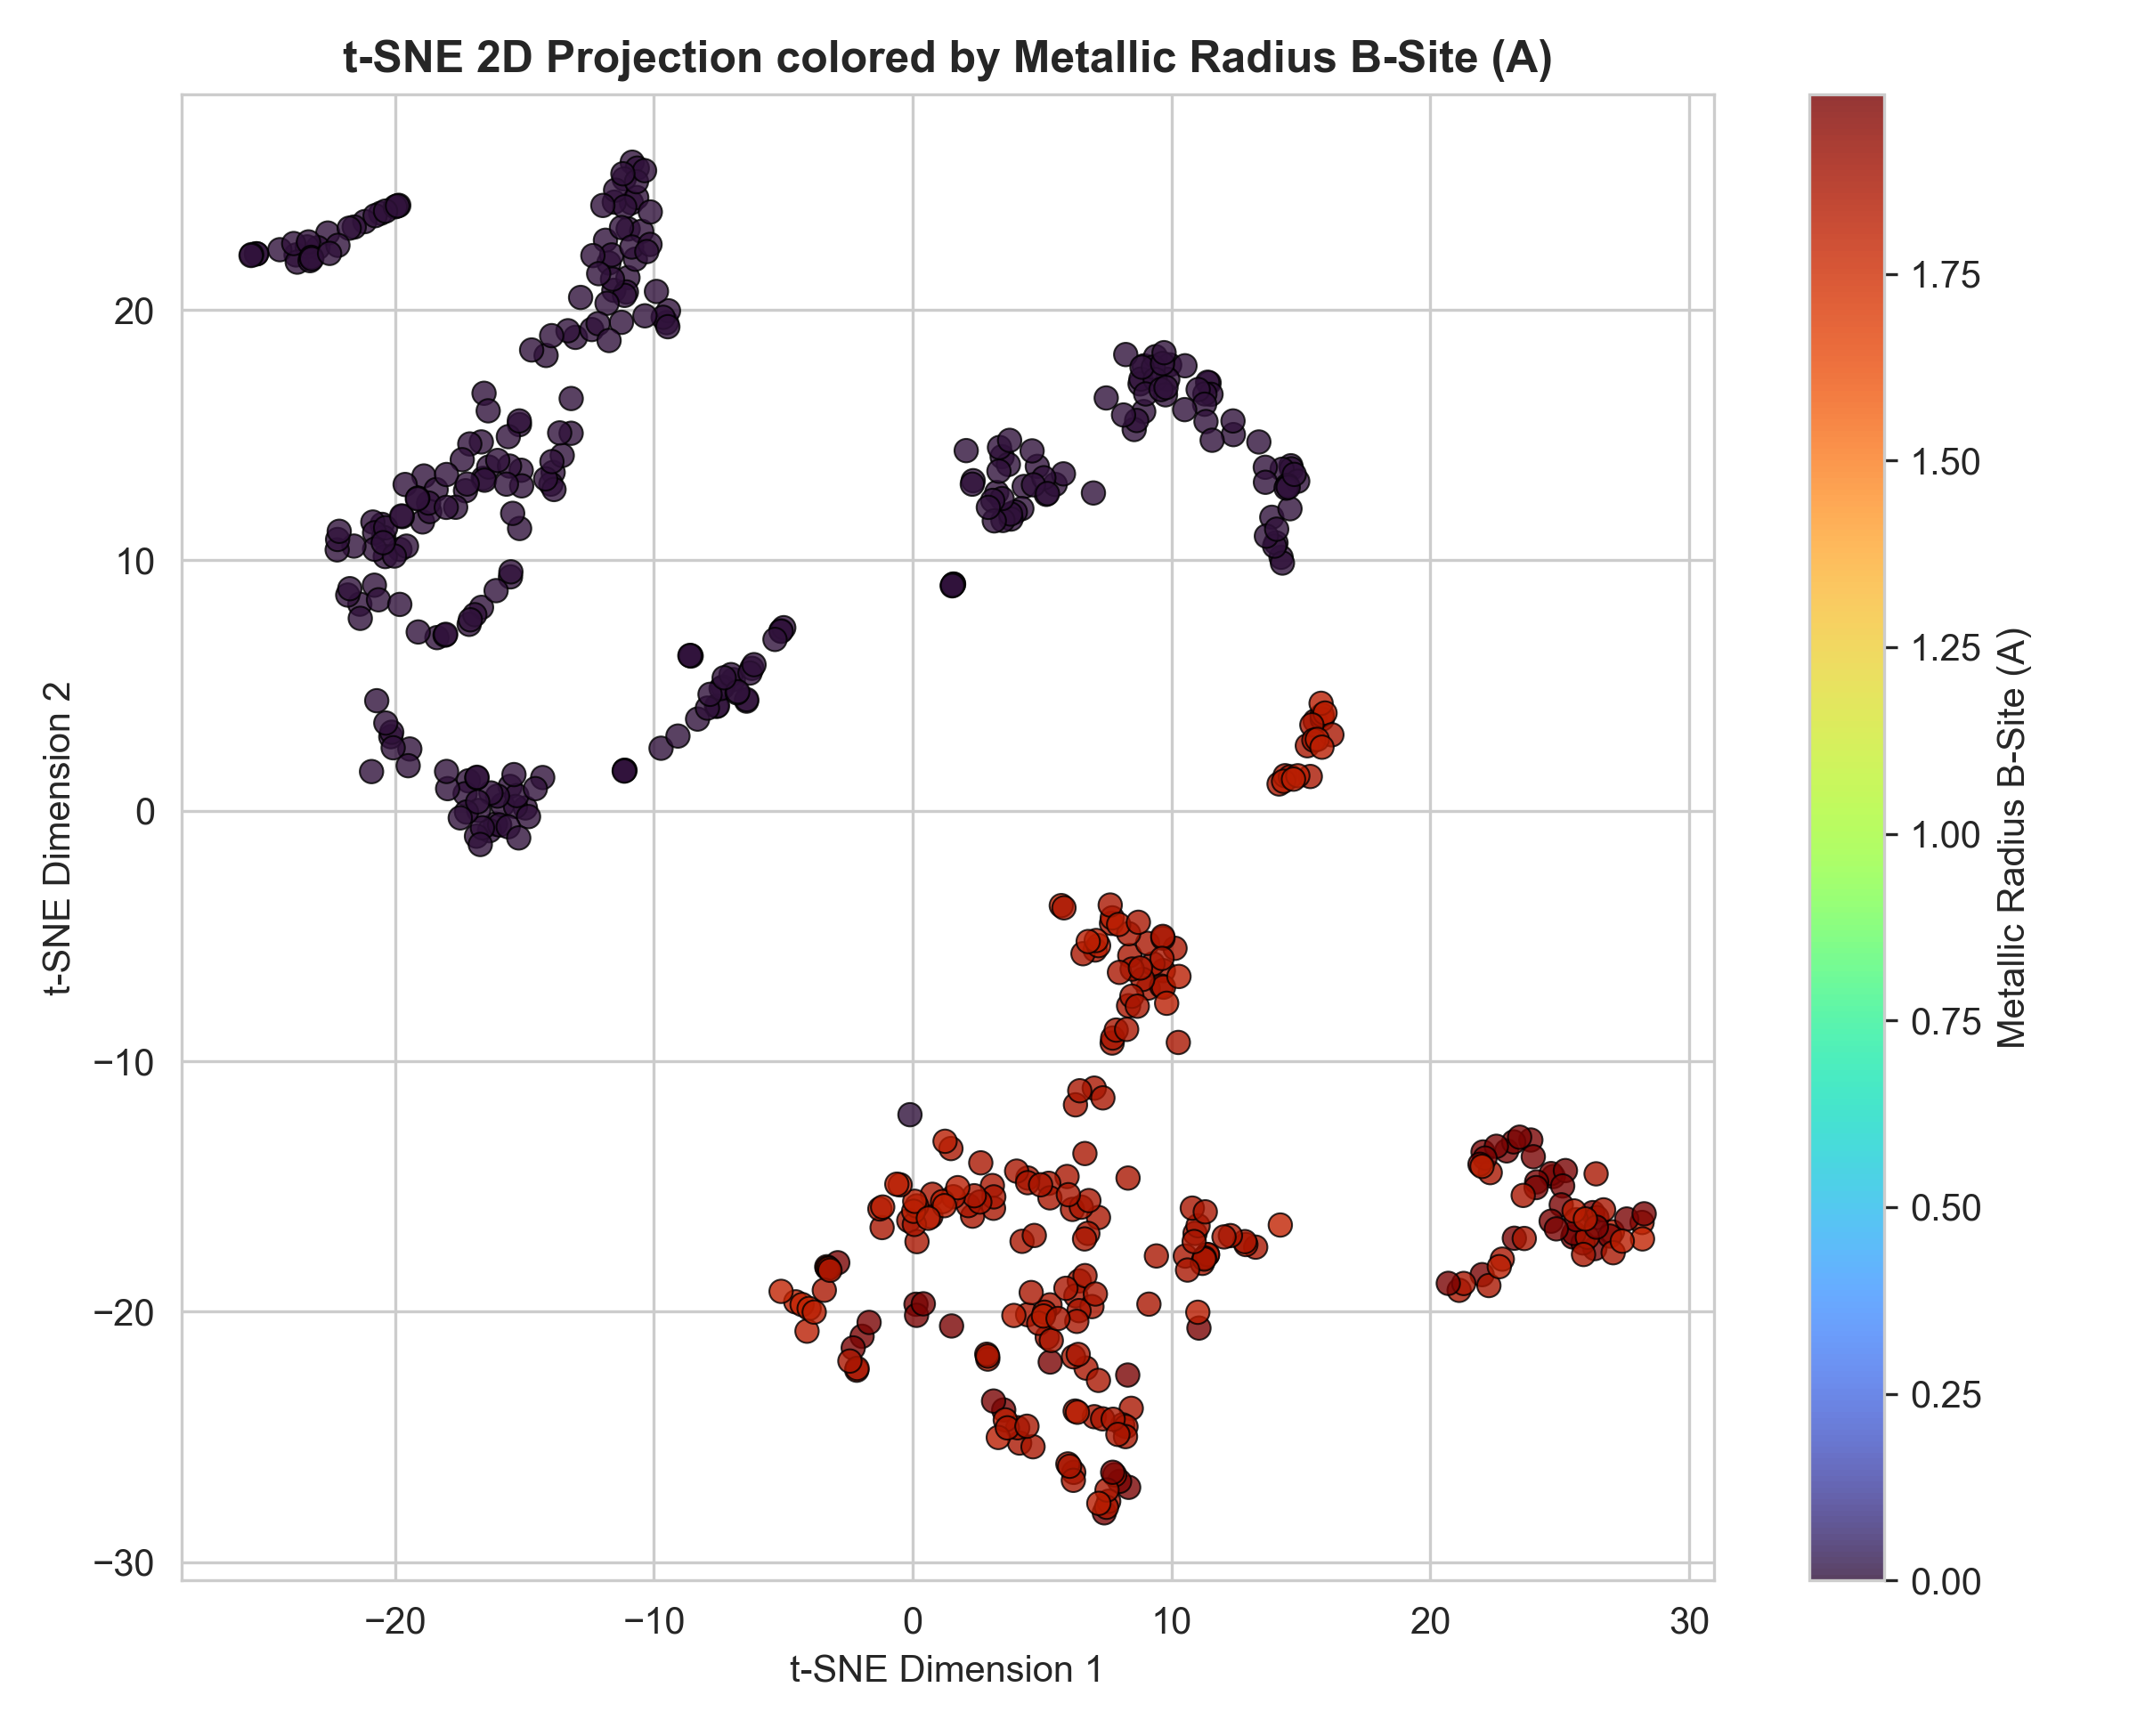
\includegraphics[width=0.65\textwidth]{3_2d_mr2.png}
  \caption{t-SNE projection of the 3D VAE latent space colored by Metallic Radius B-Site (Å).}
  \label{fig:tsne_mr2}
\end{figure}

From the generated graphs, it is clear that Band Gap, Energy Above Hull, Formation Energy and Total Magnetization display an observable gradient. This is an indicative of underlying patterns. Hence, we proceeded with prediction of specifically these properties.

\subsection{Stage 3: Finding Predictability Limits}
It is crucial to know the upper limit of predictability of these properties before we run them through interpretable machine learning models which are generally less expressive and weaker than deep learning or traditional machine learning models. The baseline accuracy and $R^{2}$ values from the deep learning/machine learning models would help us evaluate how close our interpretable models are to the deep learning/machine learning models.

For that, we deployed both Linear and Non-Linear models. For linear models, we went with OLS, Ridge and Lasso regression algorithms. While for non-linear models, we went with Gradient-(GB) Boosted Trees.

The Linear models quickly helped us identify as to which features have non-zero linear coefficients which corresponds to a mathematically percieved correlation to a certain output, be it linear or non-linear. It helped us easily discard the features that have absolutely zero correlation and could only pose as compuational overhead or noise during further analysis.

From linear regression and Gradient Boosted Trees, we got these upper limits:

\begin{table}[H]
\centering
\caption{Model Performance ($R^2$) and MAE across OLS, Ridge, Lasso, and Gradient Boosting (GB)}
\label{tab:regressions}
\footnotesize
\setlength{\tabcolsep}{1.5pt}
\begin{tabular*}{\textwidth}{@{\extracolsep{\fill}}l c c c c c c c c}
\toprule
& \multicolumn{2}{c}{\textbf{OLS}} & \multicolumn{2}{c}{\textbf{Ridge (CV)}} & \multicolumn{2}{c}{\textbf{Lasso (CV)}} & \multicolumn{2}{c}{\textbf{Gradient Boosting}} \\
\cmidrule(lr){2-3} \cmidrule(lr){4-5} \cmidrule(lr){6-7} \cmidrule(lr){8-9}
\textbf{Target Property} & $R^2$ & MAE & $R^2$ & MAE & $R^2$ & MAE & $R^2$ & MAE \\
\midrule
Formation Energy ($\Delta E_f$) & 0.6169 & 0.1766 & 0.6227 & 0.1772 & \textbf{0.6263} & 0.1778 & 0.6247 & 0.1371 \\
Total Magnetization ($M$) & \textbf{0.6019} & 2.7835 & 0.5960 & 2.7881 & 0.6009 & 2.7699 & 0.6061 & 2.8001 \\
Band Gap ($E_g$) & -0.2372 & 0.7678 & -0.2342 & 0.7672 & \textbf{-0.2090} & 0.7685 & 0.1808 & 0.6438 \\
Energy Above Hull ($E_{\text{hull}}$) & \textbf{0.3610} & 0.0464 & 0.3491 & 0.0478 & 0.3290 & 0.0483 & 0.3424 & 0.0400 \\
\bottomrule
\end{tabular*}
\end{table}

\begin{figure}[H]
  \centering
  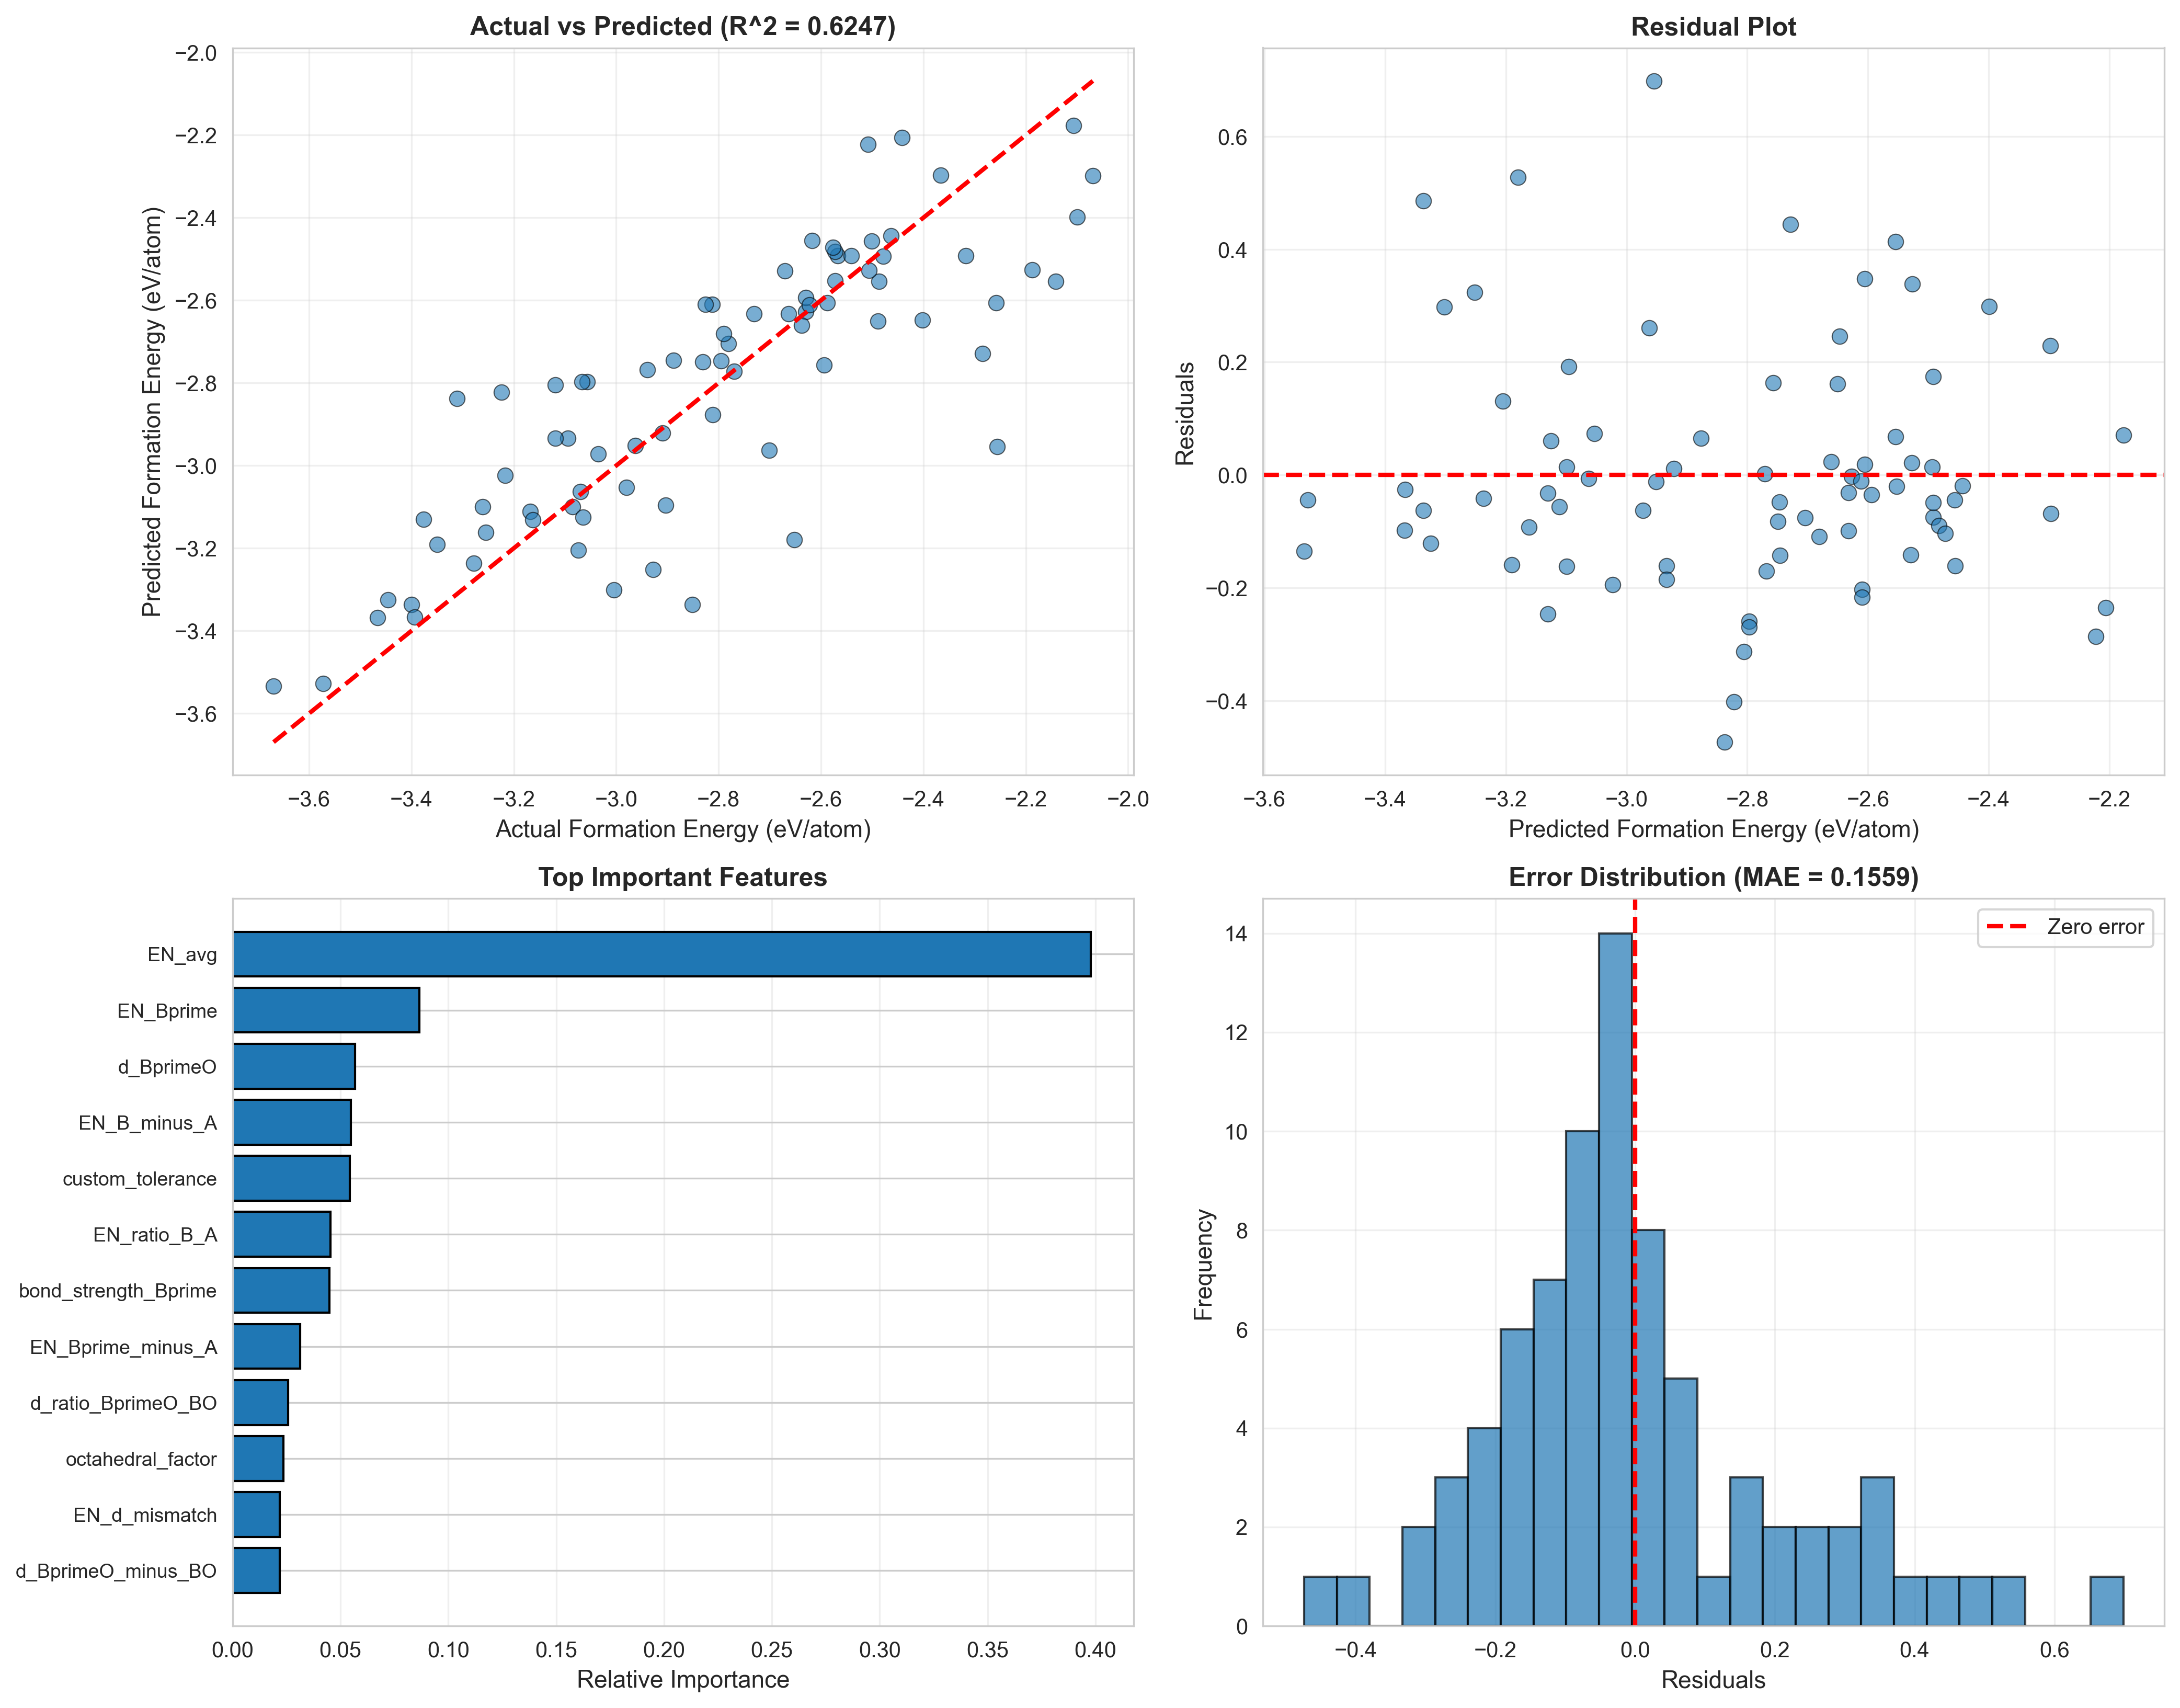
\includegraphics[width=0.85\textwidth]{formation_energy_optimized.png}
  \caption{Gradient Boosting diagnostic results for Formation Energy. The subplots show (a) actual vs. predicted values ($R^2 = 0.6247$), (b) prediction residuals, (c) the relative importance of the top 12 features (identifying $Val_{\text{avg}}$, $EN_A$, $EN_{\text{avg}}$, and $Shannon_A$ as the primary physical drivers), and (d) the residual error distribution (MAE = 0.1371 eV/atom).}
  \label{fig:feature_importance}
\end{figure}

\subsection{Stage 4: Discovering the final equations}
Using the highest weighted features from Linear Regressiona and GB Trees, we ran them through Symbolic Regression for translating the black-box systems into human-interpretable equations. We contrainted the Symbolic Regression algorithm to simple math operators: $+$, $-$, $/$, $*$, $\sqrt{x}$, and $|x|$). The algorithm was allowed to iterate for thousands of epochs until it discovered human-interpretable physical equations.

Initially, without the physical descriptors, the model came up, with huge equations such as, for the Formation energy we got (R\textsuperscript{2} = 0.137):

\begin{align*}
T_1 &= \Big| \left( \sqrt{|d_{AO}|} - 2EN_A \right) \cdot \\
    &\quad \Big[ \Big| \sqrt{\sqrt{EN_O + d_{BO} - 0.507}} \Big| + |d_{AO}| - \left( d_{BO} EN_A - 2EN_A - EN_B \right) \Big] \Big| \\
T_2 &= |EN_O| - \frac{d_{BO}}{EN_B} \\
T_3 &= \frac{\sqrt{EN_B}}{\sqrt{EN_A}} \cdot \Big[ \frac{(EN_B - d_{BO})(d_{B'O} - 0.424)}{(EN_O / d_{AO}) / \sqrt{EN_B}} + {} \\
    &\quad \sqrt{\sqrt{ \frac{EN_O}{(0.044 / EN_O) - EN_A} }} + \frac{\sqrt{d_{AO}}}{d_{AO} d_{BO}} \Big] \\
\text{Total Magnetization} &\approx (T_1 + T_2) + (T_3 + EN_A + EN_{B'})
\end{align*}

This was the generated formula for Formation energy. However, using the top physical descriptors, we came across a much cleaner equation(R\textsuperscript{2} = 0.385):

\begin{equation}
    E_f \approx EN_B - d_{B'O} + 0.892 + 0.382\frac{EN_{B'}d_{B'O}}{EN_A d_{BO}} - 0.955 EN_O
\end{equation}

The AI algorithm, was even able to come with its own tolerance factor midway:

\begin{equation*}
    \frac{EN_{B'}d_{B'O}}{EN_A d_{BO}}
\end{equation*}

However, running it for further iterations, we got an even more expressive formula (R\textsuperscript{2} = 0.533)

\begin{equation}
    \Delta E_{f} \approx t \cdot (EN_{\text{avg}} - \mu_{\text{oct}}) - d_{\text{avg}} - 0.913
\end{equation}

Yet, upon further execution, the final stable and best solution we were able to reach was(R\textsuperscript{2} = 0.6263) through Lasso Regression, just for this case:

\begin{equation}
    \boxed{\Delta E_f \approx 0.1508 \cdot Val_{\text{avg}} - 1.0197 \cdot EN_A + 0.4113 \cdot EN_{\text{avg}} - 0.2725 \cdot Shannon_A - 2.6972}
\end{equation}

The remarkable R\textsuperscript{2} of 0.6263 is far better than the expected upper limit of interpretability found by GB Tree (R\textsuperscript{2} = 0.6247).

This was repeated for the rest of parameters such as: Total Magnetization, Band Gap and Energy above Hull.

\section{Results}
Upon execution of our pipeline, this is what it came up with:

\begin{table}[H]
\centering
\small
\caption{Performance Metrics ($R^2$) Comparison across Modeling Approaches}
\label{tab:metrics_comparison}
\begin{tabularx}{\textwidth}{l *3{>{\centering\arraybackslash}X}}
\toprule
\textbf{Target Property} & \textbf{Best Linear $R^2$} & \textbf{GB $R^2$ Ceiling} & \textbf{Symbolic Regression $R^2$} \\
\midrule
Formation Energy ($\Delta E_f$) & 0.6263 (Lasso) & 0.6247 & 0.5330 \\
Total Magnetization ($M$) & 0.6019 (OLS) & 0.6061 & \textbf{0.6281} \\
Energy Above Hull ($E_{\text{hull}}$) & 0.3610 (OLS) & 0.3424 & \textbf{0.3985} \\
Band Gap ($E_g$) & -0.2090 (Lasso) & 0.1808 & \textbf{-0.1467} \\
\bottomrule
\end{tabularx}
\end{table}

\begin{table}[H]
\centering
\small
\caption{Best Discovered Physical Equations and Model Parameters}
\label{tab:best_equations}
\begin{tabularx}{\textwidth}{l X >{\raggedright\arraybackslash}p{2.8cm} c}
\toprule
\textbf{Target Property} & \textbf{Best Discovered Equation} & \textbf{Method} & \textbf{Best $R^2$} \\
\midrule
Formation Energy ($\Delta E_f$) & $\Delta E_f \approx 0.1508 \, Val_{\text{avg}} - 1.0197 \, EN_A + {}$ \newline $\quad 0.4113 \, EN_{\text{avg}} - 0.2725 \, Shannon_A - 2.6972$ & Linear Regression (Lasso) & 0.6263 \\
\addlinespace
Total Magnetization ($M$) & $M \approx \Big| \frac{t}{E_{\text{GNN}}} + E_{\text{GNN}} + EN_{\text{avg}} + {}$ \newline $\quad \Big| \frac{EN_{\text{avg}}}{E_{\text{GNN}}} + E_{\text{GNN}} + 2 \, EN_{\text{avg}} + M_{\text{abs}} - 0.249 \Big| \Big|$ & Symbolic Regression & 0.6281 \\
\addlinespace
Energy Above Hull ($E_{\text{hull}}$) & $E_{\text{hull}} \approx -0.142 \cdot E_{\text{GNN}}$ & Symbolic Regression & 0.3985 \\
\addlinespace
Band Gap ($E_g$) & $E_g \approx E_{\text{GNN}} + 0.980$ & Symbolic Regression & -0.1467 \\
\bottomrule
\end{tabularx}
\end{table}

\clearpage

\section{Discussion}
From the results, it was clear – that even among the chosen parameters that we set out for modelling, some parameters could not be distilled into an explainable equation.
Formation Energy and Total Magnetization had very high $R^2$ ($> 0.5$) values, indicating that the AI-generated equations were able to predict their value for each perovskite to a high accuracy. It signified that the generated mathematical model very closely approximates the hidden quantum effects that are taking place inside the perovskite crystal lattice.

However, Energy Above Hull, had low R\textsuperscript{2}(\(\sim\)0.3985) values, indicating that, while the mathematical model was able to model the equation well, it could only correctly predict 39.85\% of the entire dataset. Nonetheless, the mathematical model found by Symbolic Regression, outperformed Linear Regression(OLS), which indicates a successful capture of non-linearities of the crystal lattice.

For Band Gap, the R\textsuperscript{2} was less than 0, which signified that the generated mathematical model could not at all explain any data from the dataset. Gradient boosting was able to come up with R\textsuperscript{2} = 0.1818, which is incredibly low. This was primarily due to the ML models being forced to map ground-state descriptors to their excited state -- which is a fundamental boundary, since it requires descriptors such as representations of orbital symmetry and high-fidelity many-body data.

\section{Conclusion}
From the results, it is clear that machine learning approaches display a promising direction towards explainable and affordable calculation of properties of perovskites. Our success in predicting Formation Energy and Total Magnetization is an implication that, better descriptors are crucial for evolving better solutions. Symbolic regression when combined with proper feature analysis proved to be extremely helpful in generating human interpretable equations that inherently encodes quantum processes, which otherwise would have been extremely different and time consuming through bare experiments.

In future, we believe that the results could be improved through better quantum descriptors and longer Symbolic Regressions runs. Furthermore, running them on a far more broader set of equations and with better heuristics, a better equation can be expected. In particular, enhancing the connection with 3D spatial features and graph neural networks embeddings could allow filling the gap that currently exists in the ability of predicting such complicated excited state property as the electronic band gap. Overall, this work provides the foundation for a scalable approach to materials informatics based on the autonomous discovery of the fundamental laws of multi-element crystalline materials.

\begin{thebibliography}{10}

\bibitem{green2014emergence}
M.~A. Green, A.~Ho-Baillie, and H.~J. Snaith.
\newblock {The emergence of perovskite solar cells}.
\newblock {\em Nature Photonics}, 8(7):506--514, 2014.

\bibitem{pacchioni2021highly}
G.~Pacchioni.
\newblock {Highly efficient perovskite LEDs}.
\newblock {\em Nature Reviews Materials}, 6(2):108, 2021.

\bibitem{gu2016flexible}
C.~Gu and J.-S. Lee.
\newblock {Flexible Hybrid Organic–Inorganic Perovskite Memory}.
\newblock {\em ACS Nano}, 10(5):5413--5418, 2016.

\bibitem{li2025design}
Y.~Li, Y.~Ding, J.~Sun, et~al.
\newblock {Design Strategies and Emerging Applications of Perovskite-Based Sensors}.
\newblock {\em SmartMat}, 6(3):e12002, 2025.

\bibitem{nguyen2021hexagonal}
L.~T. Nguyen and R.~J. Cava.
\newblock {Hexagonal Perovskites as Quantum Materials}.
\newblock {\em Chemical Reviews}, 121(5):2935--2965, 2021.

\bibitem{ali2024elastic}
S.~Ali, et~al.
\newblock {Elastic, electronic and optical properties of double perovskites $Rb_2XCrCl_6$ (X=K, Na) via DFT study}.
\newblock {\em Journal of Physics and Chemistry of Solids}, 182:111479, 2024.

\bibitem{goldschmidt}
V.~M. Goldschmidt.
\newblock {Die Gesetze der Krystallochemie}.
\newblock {\em Naturwissenschaften}, 14(21):477--485, 1926.

\bibitem{shannon}
R.~D. Shannon.
\newblock {Revised effective ionic radii and systematic studies of interatomic distances in halides and chalcogenides}.
\newblock {\em Acta Crystallographica Section A}, 32(5):751--767, 1976.

\bibitem{jamshaid2023investigation}
S.~Jamshaid, S.~Ali, and M.~A. Khan.
\newblock {Investigation of cubic $K_2NaXBr_6$ (X=Sc, Y) double perovskites for optical and thermoelectric devices}.
\newblock {\em Journal of Physics and Chemistry of Solids}, 178:111341, 2023.

\bibitem{materialsproject}
A.~Jain, S.~P. Ong, W.~H. Gierer, et~al.
\newblock {Commentary: The Materials Project: A materials genome approach to accelerating materials innovation}.
\newblock {\em APL Materials}, 1(1):011002, 2013.

\bibitem{zhang2025efficient}
F.~Zhang, L.~Fu, W.~Gao, P.~Zhang, and J.~Zhao.
\newblock {Efficiently charting the space of mixed vacancy-ordered perovskites by machine-learning encoded atomic-site information}.
\newblock {\em npj Computational Materials}, 11(1):45, 2025.

\bibitem{chgnet}
B.~Deng, P.~Zhong, K.~Jun, et~al.
\newblock {CHGNet as a pretrained universal neural network potential for charge-informed atomistic modeling}.
\newblock {\em Nature Machine Intelligence}, 5(9):1031--1041, 2023.

\end{thebibliography}

\end{document}